%%
\documentclass[manuscript,screen,review, 12pt, nonacm]{acmart}
\let\Bbbk\relax % Fix for amssymb clash 
\usepackage{standalone}
\usepackage{vmlmacros}
\AtBeginDocument{%
  \providecommand\BibTeX{{%
    \normalfont B\kern-0.5em{\scshape i\kern-0.25em b}\kern-0.8em\TeX}}}
\usepackage{outlines}
\setlength{\headheight}{14.0pt}
\setlength{\footskip}{13.3pt}
\begin{document}
\title{An Alternative to Pattern Matching, Inspired by Verse}

\author{Roger Burtonpatel}
\email{roger.burtonpatel@tufts.edu}
\affiliation{%
  \institution{Tufts University}
  \streetaddress{419 Boston Ave}
  \city{Medford}
  \state{Massachusetts}
  \country{USA}
  \postcode{02155}
}

% \author{Norman Ramsey}
% \email{nr@cs.tufts.edu}
% \affiliation{%
% \institution{Tufts University}
% \streetaddress{177 College Ave}
% \city{Medford}
% \state{Massachusetts}
% \country{USA}
% \postcode{02155}
% }

% \author{Milod Kazerounian}
% \email{milod.mazerouniantufts.edu}
% \affiliation{%
% \institution{Tufts University}
% \streetaddress{177 College Ave}
% \city{Medford}
% \state{Massachusetts}
% \country{USA}
% \postcode{02155}
% }

\renewcommand{\shortauthors}{Burtonpatel et al.}

\begin{abstract}

Pattern matching appeals to functional programmers for its expressiveness and
good cost model via compilation to a decision tree, but it can fail to
succinctly express certain computations. Extensions to pattern matching aim to
shore up its weaknesses, but they are not unified across popular programming
languages. By contrast, equations in Verse are both expressive and succinct,
with no obvious need for extensions; however, Verse's cost model is a challenge.
\VMinus, a core language that uses Verse's equations, can be compiled to a
decision tree. \VMinus\ also subsumes \PPlus, a core language with three popular
extensions to pattern matching. 
  \end{abstract}

\maketitle
    
% \1 Title
% \1 Abstract 
% \1 Acknowledgements - maybe later? 
% \1 TOC 

% \1 Chapter 1: My thesis 
% \textbf{The thesis: Verse's equations subsume pattern matching with popular
% extensions at no extra runtime cost. This goes in the ABSTRACT. And the
% INTRODUCTION.}
\documentclass[manuscript,screen,review, 12pt, nonacm]{acmart}
\let\Bbbk\relax % Fix for amssymb clash 
\usepackage{vmlmacros}

\begin{document}

\section{Introduction}
% Subjects: Pattern matching and Equations 

Perhaps the most beloved tool among functional programmers for examining and
deconstructing data is pattern matching. 
% It does so implicitly by matching constructed data
% directly against a number of possible forms.
% Maybe combine? 
Pattern matching is also an established and well-researched topic
\citep{wadler1987views, macqueen1985tree, burton1993pattern, palao1996new,
maranget, bpc}. It is appreciated by programmers and researchers alike for two
main reasons: It enables \it{implicit} data deconstruction, and it has a
desirable cost model. Specifically (regarding the latter), pattern matching can
be compiled to a \it{decision tree}, a data structure that enforces linear
runtime performance by guaranteeing no part of the data will be examined more
than once.~\citep{maranget}

However, pattern matching cannot express certain common computations succinctly,
forcing programmers who wish to express these computations to duplicate code,
nest \it{case} expressions, and create multiple points of truth. To mitigate
this, designers of popular programming languages have introduced \it{extensions}
to pattern matching (Section~\ref{extensions}). 

Extensions strengthen pattern matching, but they are not standardized, so each
popular programming language with pattern matching features its own unique suite
of extensions. Extensions are subject to the discretion of the individual
language designer, not ubiquitous. Rather than continuing to extend pattern
matching \it{ad hoc}, a worthwhile goal could be to find an alternative that
doesn't need extensions. A tempting possibility was introduced last year by the
programming language Verse~\citep{verse}. In Verse, a programmer can deconstruct
data using a different tool the language offers: \it{equations}. Equations are
expressive and flexible, and it appears that they can express everything that
pattern matching can, including with popular extensions. 

But a full implementation of Verse is complicated, cost-wise. Verse is a
functional logic programming language, and expressions can backtrack at runtime
and return multiple results, both of which are hard to predict in their costs. 

% A worthwhile goal could be to harmonize the expressive quality of Verse's
% equations with the decision tree property of patterns.

\bf{In this thesis, I show} that the expressive quality of Verse's equations and
the decision-tree property of patterns can be combined in a single language.
Since the language is a streamlined adaptation of Verse with a reduced feature
set, I call it \VMinus (“V minus”). 
% I also show that \VMinus subsumes pattern matching with popular extensions. 

To support this claim, I have formalized \VMinus with a big-step operational
semantics (Section~\ref{vminus}), I have formalized decision trees into a core
language \D (“D”) with a big-step operational semantics (Section~\ref{d}), 
% I have formalized pattern matching in a core language \PPlus (“P plus”) with a
% big-step operational semantics (Section~\ref{pplus}),
I have formalized a translation from \VMinus to \D (Sections \ref{vminustod}),
and I have implemented both languages in Standard ML. 

\end{document}
\documentclass[manuscript,screen,review, 12pt, nonacm]{acmart}
\let\Bbbk\relax % Fix for amssymb clash 
\usepackage{vmlmacros}
\AtBeginDocument{%
  \providecommand\BibTeX{{%
    \normalfont B\kern-0.5em{\scshape i\kern-0.25em b}\kern-0.8em\TeX}}}
\usepackage{outlines}
\setlength{\headheight}{14.0pt}
\setlength{\footskip}{13.3pt}
\title{An Alternative to Pattern Matching, Inspired by Verse}
\author{Roger Burtonpatel}
\email{roger.burtonpatel@tufts.edu}
\affiliation{%
  \institution{Tufts University}
  \streetaddress{419 Boston Ave}
  \city{Medford}
  \state{Massachusetts}
  \country{USA}
  \postcode{02155}
}
\begin{document}



\section{Pattern Matching and equations}
\label{pmandequations}

In this section I'll flush out the definitions, forms, and tradeoffs of pattern
matching and equations. This will inform the compromises I make in \VMinus\ down
the line in Section~\ref{vminus}.

\subsection{Pattern matching}
\label{pmoverobservers}

% \1 What is pattern matching 

Pattern matching lets programmers examine and deconstruct data by matching them
against patterns. When a pattern $p$ matches with a value $v$, it can produce
bindings for any sub-values of $v$. 

Why use pattern matching? What could programmers use instead? One tool a
programmer might use to deconstruct data is \it{observers}[cite- Liskov and
Guttag]: functions that explicitly inquire a piece of data's structure and
manually extract its components. Examples of observers in functional programming
languages include Scheme's \tt{null?}, \tt{car}, and \tt{cdr}, and ML's
\tt{null}, \tt{hd}, and \tt{tl}. But many function programmers favor pattern
matching. I claim to know a reason why: \it{code written using pattern matching
and its extensions has superior properties to code written using observers}.
I've listed these below, and I'll refer to them as the Nice Properties from here
on out: 
\bf{\begin{enumerate}
    \item With pattern matching, code more closely resembles algebraic laws. 
    \label{p1}
    \item With pattern matching, it's easier to avoid duplicating code.
    \label{p2}
    \item Pattern matching plays nicer with user-defined types. 
    \label{p3}
    \item Pattern matching militates toward naming important intermediate
    values. \nolinebreak
    \label{p4}
    \item With pattern matching, a compiler may be able to tell if the code
    omits an important case. 
    \label{p5}
\end{enumerate}}
I'll demonstrate how pattern matching creates code that demonstrates the Nice
Properties, even in a tiny example. Consider a \it{shape} datatype in Standard
ML, which represents shapes by their side lengths: 

\medskip 
\begin{minipage}[t]{\textwidth}
    \begin{verbatim}
        datatype shape = SQUARE of real 
                       | TRIANGLE of real * real 
                       | TRAPEZOID of real * real * real
\end{verbatim}
\end{minipage}
\medskip 

Let's define an \tt{area} function on \it{shape}s, with this type and these
algebraic laws: 

\medskip 
\begin{minipage}[t]{\textwidth}
    \begin{verbatim}
        area : shape -> real 
        (* area (SQUARE s)              == s * s 
           area (TRIANGLE (w, h))       == 0.5 * w * h
           area (TRAPEZOID (b1, b2, h)) == 0.5 * b1 * b2 * h
        *)
\end{verbatim}
\end{minipage}
\medskip 

Now consider two implementations of \tt{area}, one with observers and one with
pattern matching, in Figure~\ref{fig:area}.

    \begin{figure}[H]
      \begin{minipage}[t]{0.7\textwidth}
        \begin{verbatim}
fun area sh =
  if isSquare sh
  then sqSide sh * sqSide sh
  else if isTriangle sh 
  then 0.5 * triW sh * triH sh
  else 0.5 * traB1 sh * traB2 sh * traH sh
            \end{verbatim}
            \Description{An implementation of area observers}
        \subcaption{\tt{area} with observers}
            \label{fig:observerarea} 
      \end{minipage}
      \vfill
      \begin{minipage}[t]{0.7\textwidth}
        % \centering 
        \begin{verbatim}
fun area sh =
  case sh 
    of SQUARE s              => s * s
     | TRIANGLE (w, h)       => 0.5 * w * h
     | TRAPEZOID (b1, b2, h) => 0.5 * b1 * b2 * h
                \end{verbatim}
       \Description{An implementation of area using implicit deconstruction via
       patterns.}
       \vspace{2.2em}
       \subcaption{\tt{area} with pattern matching}
       \label{fig:pmarea}
      \end{minipage}
      \caption{Implementing \tt{area} using observers is tedious, and the code
      doesn't look like the algebraic laws. Using pattern matching makes an
      equivalent implementation more appealing.}
      \label{fig:area}
    \end{figure}

    Implementing the observers \tt{isSquare}, \tt{isTriangle}, \tt{sqSide},
    \tt{triW}, \tt{traB1}, \tt{traB2}, and \tt{traH} is left as an
    (excruciating) exercise to the reader. 
    
    If that prospect doesn't convince you that pattern matching avoids a lot of
    the problems that observers have, let's see how each of our Nice Properties
    holds up in \tt{area}: 
    
    \begin{enumerate}
        \item[\bf{(1)}] \ref{fig:pmarea}, which uses pattern matching, more
        closely resembles the algebraic laws for \tt{area}. Good! 
        \item[\bf{(2)}] \ref{fig:observerarea} had to call observers like
        \tt{squareSide} multiple times, and each observer needs \tt{sh} as an
        argument. \ref{fig:pmarea} was able to extract the \tt{shape}s' internal
        values with a single pattern, and the name \tt{sh} is not duplicated
        anywhere in its body. Again, \ref{fig:pmarea} wins. 
        \item[\bf{(3)}] Where did \tt{isSquare}, \tt{sqSide}, and all the other
        observers come from? To even \it{implement} \ref{fig:observerarea}, a
        programmer has to define a whole new set of observers for \tt{shape}s!
        Most programmers find this tiresome indeed. \ref{fig:pmarea} did not
        have to do any of this. 
        \item[\bf{(4)}] To extract the internal values, \ref{fig:pmarea} had to
        name them, and their names serve as documentation. 
        \item[\bf{(5)}] If the user adds another value constructor to
        \tt{shape}- say, \tt{CIRCLE}, \ref{fig:observerarea} will not cause the
        compiler to complain, and if it's passed a \tt{CIRCLE} at runtime, the
        program will likely crash! In \ref{fig:pmarea}, the compiler will warn
        the user of the possibility of a \tt{Match} exception, and even tell
        them that they must add \tt{CIRCLE} to rule out this possibility. 
    \end{enumerate}

    Having had the chance to compare Figures \ref{fig:observerarea}
    and~\ref{fig:pmarea}, if you moderately prefer the latter, that's good: most
    functional programmers- in fact, most \it{programmers}- likely do as well. 

    Figure~\ref{fig:pmarea} provides an opportunity to introduce a few terms
    that are common in pattern matching. \ref{fig:pmarea}~is a classic example
    of where pattern matching most commonly occurs: within a case expression.
    Case expressions test a \it{scrutinee} (\tt{sh} in~\ref{fig:pmarea}) against
    a list of patterns (\tt{SQUARE s}, etc.). When the result of evaluating the
    scrutinee matches with a pattern, the program evaluates the right-hand side
    of the respective branch (\tt{s * s}, etc.) within the case
    expression.\footnote{OCaml, which you'll see in future sections, calls case
    \tt{match}. Some literature\cite{guardproposal} calls this a \it{head
    expression}. I follow Ramsey's\cite{bpc} and Maragnet's\cite{maranget}
    example in calling the things \it{case} and \it{scrutinee}. Any of these
    terms does the job.} 
% \1 Pattern matching has these properties, observers do not. 

\subsection{Popular extensions to pattern matching}
\label{extensions}

    Extensions to pattern matching simplify cases that are otherwise
    troublesome. Specifically, extensions help restore the Nice Properties in
    cases where pattern matching fails to satisfy them. 
    
    In this section, I illustrate several such instances of exactly this, and
    demonstrate how extensions help programmers write code that adheres to the
    Nice Properties. The three extensions I describe are those commonly found in
    the literature and implemented in common compilers: side conditions, pattern
    guards, and or-patterns. 
    
    For the sake of comparison, I coin the term \it{bare pattern matching} to
    denote pattern matching \it{without} extensions: in bare pattern matching,
    the only syntactic forms of patterns are names and applications of value
    constructors to zero or more patterns. 


% Subject: Extensions to pattern matching. 

\subsubsection{Side conditions}

    First, I illustrate why programmers want \it{side conditions}, an extension
    to pattern matching common in most popular functional programming languages,
    including OCaml, Erlang, Scala, and~Haskell\footnote{I use the term \it{side
    conditions} to refer to a pattern followed by a boolean expression. Some
    languages call this a \it{guard}, which I use to describe a different, more
    powerful extension to pattern matching in Section~\ref{guards}.  
    Technically, Haskell \it{only} has guards, but they subsume side conditions,
    so I hand-wavingly say that it does have side conditions.}. 
    
    Let's dive in! I'll define a (rather silly) function \tt{exclaimTall} in
    OCaml on \tt{shape}s. I'll have to translate our \tt{shape} datatype to
    OCaml, and while I'm at it, I'll write the type and algebraic laws for
    \tt{exclaimTall}:

    \begin{minipage}[t]{\textwidth}        
        \centering 
        \begin{verbatim}

type shape = Square of float 
           | Triangle of float * float
           | Trapezoid of float * float * float

exclaimTall : shape -> string 
(*
exclaimTall (Square s)              == "Wow! That's a tall square!", 
                                        where s > 100.0
exclaimTall (Triangle (w, h))       == "Goodness! Towering triangle!",
                                        where h > 100.0
exclaimTall (Trapezoid (b1, b2, h)) == "Zounds! Tremendous trapezoid!", 
                                        where h > 100.0
exclaimBigArea sh                   == "Your shape is small.", 
                                        otherwise
*)
    \end{verbatim}
    \end{minipage}

    Armed with pattern matching, I'll try to implement \tt{exclaimTall} in OCaml
    (Figure~\ref{fig:ifexclaimtall}).

    \begin{figure}[ht]
        \begin{verbatim}
            let exclaimTall sh =
            match sh with 
              | Square s -> if s > 100.0 
                            then "Wow! That's a tall square!"
                            else "Your shape is small." 
              | Triangle (_, h) -> 
                            if h > 100.0 
                            then "Goodness! Towering triangle!"
                            else "Your shape is small." 
              | Trapezoid (_, _, h) -> 
                            if h > 100.0
                            then "Zounds! Tremendous trapezoid!"
                            else "Your shape is small." 
            \end{verbatim}    
        \caption{An invented function \tt{exclaimTall} in OCaml combines pattern
        matching with an \tt{if} expression, and is not very pretty.}   
        \Description{An implementation of a function exclaimTall in OCaml, which
        uses pattern matching and an if statement.}
        \label{fig:ifexclaimtall}
    \end{figure}
    
    Here, I'm using the special variable \tt{\_}- a wildcard pattern- to
    indicate that I don't care about the bindings of a pattern. 

    I (and hopefully you, the reader) are not thrilled with this code. It gets
    the job done, but it fails to adhere to Nice Properties \ref{p1}
    and~\ref{p2}: the code does not look like the algebraic laws, and it
    duplicates right-hand side, \tt{"Your shape is small"}, three times. I find
    the code unpleasant to read, too: the actual “good” return values of the
    function, the exclamatory strings, are gummed up in the middle of the
    \tt{if-then-else} expressions.
    
    Fortunately, this code can be simplified by using the \tt{shape} patterns
    with a \it{side condition}, i.e., a syntactic form for “match a pattern
    \it{and} a boolean condition.” The \tt{when} keyword in OCaml provides such
    a form, as seen in Figure~\ref{fig:whenexclaimtall}.
        
        \begin{figure}[]
            \begin{verbatim}
                let exclaimTall sh =
                  match sh with 
                    | Square s when s > 100.0 ->
                            "Wow! That's a tall square!"
                    | Triangle (_, h) when h > 100.0 ->
                            "Goodness! Towering triangle!"
                    | Trapezoid (_, _, h) when h > 100.0 -> 
                            "Zounds! Tremendous trapezoid!"
                    | _ ->  "Your shape is small." 
                \end{verbatim}
            \caption{With a side condition, \tt{exclaimTall} in OCaml becomes
            simpler and more adherent to the Nice Properties.} 
            \Description{An implementation of a function exclaimTall in OCaml,
            which uses pattern matching and a side condition.}
            \label{fig:whenexclaimtall}
        \end{figure}

    A side condition streamlines pattern-and-boolean cases and minimize
    overhead. And a side condition can exploit bindings that emerge from the
    preceding pattern match. For instance, the \tt{when} clauses in
    Figure~\ref{fig:whenexclaimtall} exploit names \tt{s} and \tt{h}, which are
    bound in the match of \tt{sh} to \tt{Square s}, \tt{Triangle (\_, h)}, and
    \tt{Trapezoid (\_, \_, h)}, respectively. 

    A side condition can incorporate an extra “check”- in this case, a boolean
    expression- within a pattern. But side conditions have a limitation. The
    check can make a decision based off of an expression evaluating to \tt{true}
    or \tt{false}. But it can't make a decision based off an arbitrary pattern
    match, and it can't bind names for the programmer to use in the right-hand
    side. In the next section, I showcase when this limitation matters, and how
    another extension addresses it. 

    \subsubsection{Pattern guards}
    \label{guards}

    To highlight a common use of pattern guards, I modify an example from Erwig
    \& Peyton-Jones\cite{guardproposal}, the proposal for pattern guards in GHC.
    Suppose I have an OCaml abstract data type of finite maps, with a lookup
    operation: 

    \medskip
    \begin{minipage}[t]{\textwidth}
        \centering 
        \begin{verbatim}
            lookup : finitemap -> int -> int option
        \end{verbatim}
    \end{minipage}
    
    Let's say I want to perform three successive lookups, and call a “fail”
    function if either of them returns \tt{None}. I want a function with 
    this type and algebraic laws: 

    \begin{minipage}[t]{\textwidth}
        \centering 
        \begin{verbatim}
          

            tripleLookup : finitemap -> int -> int

            tripleLookup rho x == z, where 
                                       lookup rho x == Some w
                                       lookup rho w == Some y
                                       lookup rho y == Some z
            tripleLookup rho x == handleFailure x, otherwise
            
            handleFailure : int -> int 
            (* handleFailure's implementation is unimportant.
               handleFailure (x : int) = ... some error-handling ... -> x *)  

        \end{verbatim}
    \end{minipage}

    To express this computation succinctly, the program needs to make decisions
    based on how successive computations match with patterns, but neither bare
    pattern matching nor side conditions don't give that flexibility. 
    
    Side conditions don't appear to help here, so I'll try with bare pattern
    matching. Figure~\ref{fig:pmtriplelookup} shows how I might implement
    \tt{tripleLookup} as such. 

    \begin{figure}[ht]
        \begin{verbatim}

          let tripleLookup (rho : finitemap) (x : int) =
              match lookup rho x with Some w -> 
                (match lookup rho w with Some y -> 
                  (match lookup rho y with Some z -> z
                  | _ -> handleFailure x)
                | _ -> handleFailure x)
              | _ -> handleFailure x
            \end{verbatim}
        \caption{\tt{tripleLookup} in OCaml with bare pattern matching breaks
                    Nice Property~\ref{p2}: avoiding duplicated code. } 
                    
        \Description{An implementation of the tripleLookup with three levels of
        nested pattern matching.}
        \label{fig:pmtriplelookup}
    \end{figure}

    Once again, the code works, but it's lost Nice Properties \ref{p2}
    and~\ref{p1} by duplicating three calls to \tt{handleFailure} and stuffing
    the screen full of syntax that distracts from the algebraic laws.
    Unfortunately, it's not obvious how a side condition could help us here,
    because we need pattern matching to extract and name internal values from
    constructed data.

    To restore the Nice Properties, I'll introduce a more powerful extension to
    pattern matching: \it{pattern guards}, a form of “smart pattern” in which
    intermediate patterns bind to expressions within a single branch of a
    \tt{case}. Pattern guards can make \tt{tripleLookup} \it{much} appear
    simpler, as shown in Figure~\ref{fig:guardtriplelookup}-- which, since
    pattern guards aren't found in OCaml, is written in Haskell.

    \begin{figure}[hbt!]  
        \begin{center}
        \begin{verbatim}
                        tripleLookup rho x
                           | Just w <- lookup rho x
                           , Just y <- lookup rho w
                           , Just z <- lookup rho y
                           = z
                        tripleLookup _ x = handleFailure x
        \end{verbatim}
        \end{center}    
    \caption{Pattern guards swoop in to restore the Nice Properties, and all is
    right again.} 
    \Description{An implementation of nameOf using pattern guards.}
    \label{fig:guardtriplelookup}
    \end{figure}

    Guards appear as a comma-separated list between the \tt{|} and the \tt{=}.
    On the left-hand side of the \tt{<-} is a pattern, and on the right is an
    expression. At runtime, the program processes a guard by evaluating the
    expression and testing if it matches with the pattern. If it does, it
    processes the next guard with any bindings introduced by processing guards
    before it. If it fails, the program skips evaluating the rest of the branch
    and falls through to the next one. As a bonus, a guard can simply be a
    boolean expression which the program tests the same way it would a side
    condition, so guards subsume side conditions! 
    
    If you need further convincing on why programmers want for guards, look no
    further than Erwig \& Peyton-Jones's \it{Pattern Guards and Transformational
    Patterns}\cite{guardproposal}, the proposal for pattern guards in GHC: the
    authors show several other examples where guards drastically simplify
    otherwise-maddening code. 
    
    The power of pattern guards lies in the ability for expressions within
    guards to utilize names bound in preceding guards, enabling imperative
    pattern-matched steps with expressive capabilities akin to Haskell's \tt{do}
    notation. It should come as no surprise that pattern guards are built in to
    GHC. 

\subsubsection{Or-patterns}

    I conclude our tour of extensions to pattern matching with or-patterns,
    which are built in to OCaml. Let's consider a final example. I have a type
    \tt{token} which represents a token in a video game and how much fun it is,
    and need to quickly know what game it's from and how fun I'd have playing
    it. To do so, I'm going to write a function \tt{game\_of\_token} in OCaml.
    Here are the \tt{token} type and the type and algebraic laws for
    \tt{game\_of\_token}. 

\begin{minipage}[t]{\textwidth}
    \centering 
    \begin{verbatim}

    type funlevel = int

    type token = BattlePass  of funlevel 
               | ChugJug     of funlevel 
               | TomatoTown  of funlevel
               | HuntersMark of funlevel 
               | SawCleaver  of funlevel
               | MoghLordOfBlood of funlevel 
               | PreatorRykard   of funlevel
               ... other tokens ...
                   

game_of_token : token -> string * funlevel

game_of_token t == ("Fortnite", f),  where t is any of 
                                      BattlePass f, 
                                      ChugJug f, or
                                      TomatoTown f
game_of_token t == ("Bloodborne", 2 * f), 
                                      where t is any of 
                                        HuntersMark f or 
                                        SawCleaver f
game_of_token t == ("Elden Ring", 3 * f), 
                                      where t is any of 
                                        MoghLordOfBlood f or  
                                        PreatorRykard f
game_of_token _ == ("Irrelevant", 0), otherwise
    \end{verbatim}
\end{minipage}        
        
        I can write code for \tt{game\_of\_token} in OCaml using bare patterns
        (Figure~\ref{fig:baregot}), but I'm dissatisfied with how it fails the
        first three (\ref{p1}, \ref{p2}, \ref{p3}) of the Nice Properties: it
        has many duplicated right-hand sides, it is visually dissimilarity to
        the algebraic laws, and the function, even though it uses pattern
        matching, doesn't really play nice with my custom type; deconstructing
        it is tedious and redundant.         
        
        \begin{figure}
            \begin{center}
                \begin{verbatim}
        let game_of_token token = match token with 
            | BattlePass f      -> ("Fortnite", f)
            | ChugJug f         -> ("Fortnite", f)
            | TomatoTown f      -> ("Fortnite", f)
            | HuntersMark f     -> ("Bloodborne", 2 * f)
            | SawCleaver f      -> ("Bloodborne", 2 * f)
            | MoghLordOfBlood f -> ("Elden Ring", 3 * f)
            | PreatorRykard f   -> ("Elden Ring", 3 * f)
            | _                 -> ("Irrelevant", 0)
                \end{verbatim}
            \end{center}    

        \caption{\tt{game\_of\_token}, with redundant right-hand sides,
        should raise a red flag.} 
        \Description{An implementation of game_of_token using bare patterns.}
        \label{fig:baregot}
        \end{figure}

        I could try to use a couple of helper functions to reduce clutter, and
        write something like Figure~\ref{fig:helpergot}. It looks ok, but I'm
        still hurting for Nice Properties \ref{p2} and \ref{p3}, and the
        additional calls hurt performance. 

        \begin{figure}
            \begin{center}
                \begin{verbatim}
                  let fortnite   f = ... complicated   ... in
                  let bloodborne f = ... complicated'  ... in
                  let eldenring  f = ... complicated'' ... in
                  match token with
                  | BattlePass f -> fortnite f
                  ... and so on ...                
                \end{verbatim}
            \end{center}    
        \caption{\tt{game\_of\_token} with helpers is somewhat better, but I'm
        not satisfied with it.} 
        \Description{An implementation of
        game_of_token using helper functions.}
        \label{fig:helpergot}
        \end{figure}

        Thankfully, an extension once again comes to the rescue.
        \it{Or-patterns} condense multiple patterns which share right-hand
        sides, and I can exploit them to restore the Nice Properties and
        eliminate much uninteresting code in Figure~\ref{fig:orgot}.

    \begin{figure}
    \begin{center}
    \begin{verbatim}
let game_of_token token = match token with 
    | BattlePass f | ChugJug f | TomatoTown f  -> ("Fortnite", f)
    | HuntersMark f | SawCleaver f             -> ("Bloodborne", 2 * f)
    | MoghLordOfBlood f | PreatorRykard f      -> ("Elden Ring", 3 * f)
    | _                                        -> ("Irrelevant", 0)
    \end{verbatim}
    \end{center}    
    \caption{Or-patterns condense \tt{game\_of\_token}
    significantly, and it is easier to read line-by-line.} 
    \Description{An
    implementation of game_of_token using or-patterns.}
    \label{fig:orgot}
    \end{figure}

    In addition to the inherent appeal of brevity, or-patterns serve to
    concentrate complexity at a single juncture and create single points of
    truth. And by eliminating helper functions, like the ones in
    Figure~\ref{fig:helpergot}, or-patterns actually boost performance.
      
    \subsubsection{Wrapping up pattern matching and extensions}
    
    Now, any pattern matching-loving functional programmer like me or (now,
    hopefully!) you knows about the extensions that make pattern matching more
    expressive and how to use them effectively. Earlier, though, you might have
    noticed a problem. Say we face a decision-making problem that obliges us to
    use all of our extensions in unison. When picking a language to do so, we
    are stuck! Indeed, no major functional language has all three of these
    extensions. Remember when we had to switch from OCaml to Haskell to use
    guards, and back to OCaml for or-patterns? The two extensions are mutually
    exclusive in Haskell and OCaml, and also Scala, Erlang/Elixir, Rust, F\#,
    and Agda\cite{haskell, ocaml, scala, erlang, elixir, rust, fsharp, agda}. 


    I find the extension story somewhat unsatisfying. At the very least, I want
    to be able to use pattern matching, with the extensions I want, in a single
    language. Or, I want an alternative that gives me the expressive power of
    pattern matching with these extensions. 

    Last year, I spotted an intriguing alternative to pattern matching:
    \it{equations}, from the Verse Calculus\cite{verse}. Equations present a
    different, yet powerful, way to write code that makes decisions and
    deconstructs data. In the next section, I'll introduce you to equations
    similarly to I how I introduced to you pattern matching. Once you're
    familiar with equations, you'll be ready to compare their strengths and
    weaknesses with those of pattern matching, and judge the compromise I
    propose. 

\subsection{Verse's equations}
    \label{verseoverobservers}

    % \1 Equations 
    Allow me to turn your attention to the equations of the Verse Calculus
    (\VC), a core calculus for the functional logic programming
    language\cite{antoy2010functional, hanus2013functional} Verse\cite{verse}.
    (For the remainder of this paper, I use “\VC” and “Verse” interchangeably.)

    Even if you read the Verse paper, \VC's equations and the paradigms of
    functional logic programming might look unfamiliar to your pattern
    matching-accustomed brains. To help ease you into familiarity with
    equations, I'll ground explanations and examples in how they relate to
    pattern matching. 

    \VC\ uses \it{equations} instead of pattern matching to test for structural
    equality and create bindings. Like pattern matching, equations scrutinize
    and deconstruct data at runtime by testing for structural equality and
    unifying names with values. Unlike pattern matching, \VC's equations can
    unify names on both left- \it{and} right-hand sides. 

    Equations in Verse take the form \it{x = e}, where \it{x} is a name and
    \it{e} is an expression. During runtime, both \it{x} and any unbound names
    in \it{e} are unified with values. Much like pattern matching, unification
    can fail if the runtime attempts to bind incompatible values or structures. 

    Equations offer a form of binding that looks like a single pattern match.
    What about a list of many patterns and right-hand sides, as in a case
    expression? For this, \VC\ has \it{choice} (\choice). The full semantics of
    choice are too complex for me to cover in this paper, but you can get away
    with knowing that choice, when combined with the \tt{one} operator, has a
    very similar semantics to case; that is, “proceed and create bindings if any
    one of these computations succeed.” 

    Let's look at what equations, \tt{one}, and choice look like in real,
    written Verse code. I've written our \tt{area} function in \VC\ extended
    with a \tt{float} type and a multiplication operator \tt{*} in
    Figure~\ref{fig:versearea}. 

    \begin{figure}[]
        \verselst
        \begin{lstlisting}[numbers=none]
$\exists$ area. area = $\lambda$ sh. 
  one {  $\exists$ x. sh   = $\langle$SQUARE, s$\rangle$; s * s
       | $\exists$ w h. sh = $\langle$TRIANGLE, w, h$\rangle$; 
              0.5 * w * h
       | $\exists$ b1 b2 h. sh = $\langle$TRAPEZOID, b1, b2, h$\rangle$; 
              0.5 * b1 * b2 * h}
        \end{lstlisting}
    \caption{\tt{area} in \VC\ uses existentials and equations rather than
    pattern matching.} 
    \Description{An implementation of area in Verse.}
    \label{fig:versearea}
    \end{figure}

    Like in the pattern-matching example in good old \ref{fig:pmarea}, the
    right-hand sides of \tt{area} are \it{guarded} by a “check;” now, the check
    is successful unification in an equation rather than a successful match on a
    pattern. Similarly, \tt{one} with a list of choices represents matching on
    any \it{one} pattern to evaluate a single right-hand side. 

    Why use equations? Let's start with a digestible claim: I prefer \VC's
    equations to observers, and I imagine many functional programmers would as
    well. To support this claim, I appeal to the Nice Properties: 

    \begin{enumerate}
      \item \tt{area} using equations looks like the algebraic laws, with the
      addition of the explicit $\exists$. It's a bit more math-y, but that might
      not be a bad thing: though it doesn't resemble the algebraic laws a
      programmer would write, it likely resembles the equations that a
      mathematician would. 
      \item \tt{area} using equations does not duplicate virtually any code. 
      \item \tt{area} using equations deconstructs user-defined types as easily
      as \ref{fig:pmarea} does with pattern matching. 
      \item \tt{area} using equations has all important internal values named
      very explicitly.
      \item This Property may not hold, because \VC\ on its own is untyped.
      Without a type system, a compiler cannot help me with non-exhaustive
      cases. However, there is no published compiler, type system or no, for
      Verse, and only when one is made available can I make this assertion. For
      this reason, and for the sake of focusing on more important details, I
      choose to proceed in my analysis of equations in \VC\ without considering
      this Property. 
    \end{enumerate}

    If you still believe these Properties to be desirable, you understand why I
    claim programmers prefer equations to observers. Now I'll make a stronger
    claim: equations are \it{at least as good as} pattern matching with popular
    extensions. How can I claim this? By appealing again to the Nice Properties!
    Do you remember how in Section~\ref{pmoverobservers}, I demonstrated how
    pattern matching had to resort to extensions to regain the Properties when
    challenging examples stole them away? In Figure~\ref{fig:verseextfuncs},
    I've implemented those examples in \VC\ (this time extended with strings,
    floats, and \tt{*}) using choice and equations. Take a look for yourself! 

    \begin{figure}[ht] 
        \begin{minipage}[h]{0.54\linewidth}
          \verselst
          \begin{lstlisting}[numbers=none, basicstyle=\tiny, xleftmargin=.2em,
                            showstringspaces=false,
                            frame=single]
$\exists$ exclaimTall. exclaimTall = $\lambda$ sh. 
  one { 
      $\exists$ s. sh = $\langle$Square s$\rangle$; 
      s > 100.0; "Wow! That's a tall square!"
    | $\exists$ w h. sh = $\langle$Triangle, w, h$\rangle$; 
      h > 100.0; "Goodness! Towering triangle!"
    | $\exists$ b1 b2 h. sh = $\langle$Trapezoid, b1, b2, h$\rangle$;
      h > 100.0; "Zounds! Tremendous trapezoid!"
    | "Your shape is small." }
            \end{lstlisting}
                \Description{exclaimTall}
        \subcaption{\tt{exclaimTall} in \VC\ }
            \label{fig:verseexclaimtall} 
        %   \vspace{4ex}
        \end{minipage}%%
        \begin{minipage}[h]{0.5\linewidth}
          \verselst
          \begin{lstlisting}[numbers=none, basicstyle=\tiny, xleftmargin=2em,
                        frame=single]
$\exists$ tripleLookup. tripleLookup = $\lambda$ rho x. 
    one { $\exists$ w. lookup rho x = $\langle$Just w$\rangle$; 
          $\exists$ y. lookup rho w = $\langle$Just y$\rangle$; 
          $\exists$ z. lookup rho y = $\langle$Just z$\rangle$;
          z
        | handleFailure x }
          \end{lstlisting}
                \Description{exclaimTall}
            \subcaption{\tt{tripleLookup} in \VC\ }
            \label{fig:versetriplelookup} 
        \vspace{4ex}
        \end{minipage} 
        \begin{minipage}[h]{\linewidth}
          \verselst
          \begin{lstlisting}[numbers=none, basicstyle=\tiny, xleftmargin=9em, 
                            frame=single, showstringspaces=false]
$\exists$ game_of_token. game_of_token = $\lambda$ token. 
  $\exists$ f. one {
         token = one { $\langle$BattlePass, f$\rangle$ | $\langle$ChugJug, f$\rangle$ | $\langle$TomatoTown, f$\rangle$}; 
           $\langle$"Fortnite", f$\rangle$
       | token = one { $\langle$HuntersMark, f$\rangle$ | $\langle$SawCleaver, f$\rangle$}; 
           $\langle$"Bloodborne", 2 * f$\rangle$
       | token = one { $\langle$MoghLordOfBlood, f$\rangle$ | $\langle$PreatorRykard, f$\rangle$}; 
           $\langle$"Elden Ring", 3 * f$\rangle$
       |   $\langle$"Irrelevant", 0$\rangle$ }
          \end{lstlisting}
                \Description{game_of_token in \VC}
        \subcaption{\tt{game\_of\_token} in \VC\ }
            \label{fig:versegot} 
        \vspace{4ex}
        \end{minipage}%% 
    \caption{Code for the \ref{pmoverobservers} functions with equations looks
    similar, and it doesn't need extensions.}
    \label{fig:verseextfuncs}
      \end{figure}
        
    The code in Figure~\ref{fig:verseextfuncs} has all the Nice Properties
    (again, disregarding the ambiguous 5th.) This is promising for \VC. If it
    rivals pattern matching with popular extensions in desirable properties, and
    \VC\ does everything using only equations and choice, it seems like the
    language is a strong option for writing code! 

    \subsection{\VC\ has a challenging cost model}
    \label{vcbadcost}

    So what's the catch? Programmers everywhere have not thrown up their hands,
    renounced pattern matching, and adopted a puritanical dogma of equations. 
    Sadly, this is not merely a matter of preference. 

    \VC's equations appear to be comparably pleasing to pattern matching in
    their brevity and expressiveness. However, full Verse allows computations
    that are problematic, cost-wise. In \VC, names (logical variables) are
    \it{values}, and can just as easily be the result of evaluating an
    expression as an integer or tuple. To bind these names, \VC, like other
    functional logic languages, relies on \it{unification} of its logical
    variables and \it{search} at runtime to meet a set of program
    constraints\cite{antoy2010functional, hanus2013functional}. Combining
    unifying logical variables with search at runtime classically requires
    backtracking, which can lead to exponential runtime
    cost\cite{hanus2013functional, wadler1985replace, clark1982introduction}. 

    % Todo: An example would be nice. Backtracking/evaluating backwards, then
    % done. 

    Pattern matching, by contrast, has a desirable cost model.
    Maranget\cite{maranget} showed that pattern matching can be compiled to a
    \it{decision tree}, a data structure that enforces linear runtime
    performance by guaranteeing no part of the scrutinee will be examined more
    than once. A decision tree, however, forbids backtracking by nature: once
    the program makes a decision based on the form of a value, it can't re-test
    it later with new information. 
    

\end{document}
\documentclass[manuscript,screen,review, 12pt, nonacm]{acmart}
\let\Bbbk\relax % Fix for amssymb clash 
\usepackage{vmlmacros}
\AtBeginDocument{%
  \providecommand\BibTeX{{%
    \normalfont B\kern-0.5em{\scshape i\kern-0.25em b}\kern-0.8em\TeX}}}
\usepackage{outlines}
\setlength{\headheight}{14.0pt}
\setlength{\footskip}{13.3pt}
\title{An Alternative to Pattern Matching, Inspired by Verse}

\author{Roger Burtonpatel}
\email{roger.burtonpatel@tufts.edu}
\affiliation{%
\institution{Tufts University}
\streetaddress{419 Boston Ave}
  \city{Medford}
  \state{Massachusetts}
  \country{USA}
  \postcode{02155}
  }
\begin{document}
  
\section{A compromise}
    I have created and implemented a semantics for three core languages that aim
    to bridge the gap between pattern matching, equations, and decision trees.
    They are \PPlus, which has pattern matching with all the above extensions,
    \VMinus, which has equations without backtracking or multiple results, and
    \D, which has decision trees. \PPlus and \VMinus serve to explore the
    design space of pattern matching and equations, while \D serves as the
    target of translation to reason about efficiency. 

    In this section, I present the three languages. Their semantics appear in
    Figures X, Y, and Z, respectively, and in Appendix A. In my design, I took
    inspiration from Verse: each of \PPlus, \VMinus, and \D has a conventional
    sub-language that is the lambda calculus extended with named value
    constructors \it{K} applied to zero or more values. I chose named value
    constructors over \VC's tuples because they look more like patterns. 
    
    Because they share a core, and to facilitate comparisons and proofs, I have
    decided to present \VMinus, \PPlus, and \D as three subsets of a single
    unifying language, whose abstract syntax is given in
    Figure~\ref{fig:unilang}. Column “Unique To” indicates which components of
    this unifying language belong to the sub-languages. For all intents and
    purposes, the three languages are distinct; it is because they all share the
    same core of lambdas, value constructors (\it{K}), names, and function
    application that I have decided to house them under the same umbrella
    figure. 
    
    Like in \VC, every lambda calculus term is valid in our languages and has
    the same semantics. Also like the lambda calculus and \VC, all three
    languages are \it{strict}, meaning expressions are always evaluated when
    they are bound to variables, and they are all untyped. Creating a type
    system for \PPlus and \VMinus is a worthy effort but is the subject of
    another paper. \D mainly exists as the target of translations, so typing it
    is neither particularly interesting nor worthwhile. 
    
    In the subsections below, I discuss each language in more detail.
    Section~\ref{futurework} goes further in analyzing how \PPlus and \VMinus
    relate to modern languages with pattern matching and to \VC respectively. 

\subsection{Introducing \PPlus}
\label{pplus}

    \PPlus packages common extensions to pattern matching with a standard core.
    In addition to bare pattern matching— names and applications of value
    constructors— the language includes pattern guards, or-patterns, and side
    conditions. You may point out that pattern guards subsume side conditions
    (yes, they do!); we include side conditions and separate them from guards
    for purpose of study. Furthermore, \PPlus introduces a new form of pattern:
    \pcommap. This allows a pattern in \PPlus be a \it{sequence} of
    sub-patterns, allowing a programmer to stuff as many patterns as they want
    in the space of a single one. I discuss the implications of this in
    Section~\ref{ppweird}.

\subsection{Formal Semantics of \PPlus}

\begin{figure}
\begin{center}
\begin{bnf}
$P$ : \textsf{Programs} ::=
$\bracketed{d}$ : definition
;;
$d$ : \textsf{Definitions} ::=
| $\tt{val}\; x\; \tt{=}\; \expr$ : bind name to expression
;;
$\expr$ : Expressions ::= 
| $v$ : literal values 
| $x, y, z$ : names
| $K\bracketed{\expr}$ : value constructor application 
| $\ttbackslash x.\; \expr$ : lambda declaration  
| $\expr[1]\; \expr[2]$ : function application 
| $\tt{case}\; \expr\; \bracketed{p\; \ttrightarrow\; \expr}$ : \it{case} expression 
| \ttbraced{$\expr$}
;;
$p$ : \textsf{Patterns} ::= $p_{1}\pbar p_{2}$ : or-pattern
| $p \tt{,} p'$ : pattern guard 
| $p\; \tt{<-}\; \expr$ : pattern from explicit expression  
| $x$ : name 
| $\tt{\_}$ : wildcard 
| $K\; \bracketed{p}$ : value constructor application 
| $\tt{when}\; \expr$
| \ttbraced{$p$}
;;
$\v$ : Values ::= $K\bracketed{\v}$ : value constructor application 
| $\ttbackslash x.\; \expr$ : lambda value 
;;
$K$ : \textsf{Value Constructors} ::=
| $\tt{true}\; \vert\; \tt{false}$ : booleans
| $\tt{A-Z}x$ : name beginning with capital letter
% | $[\tt{-}\vert\tt{+}](\tt{0}-\tt{9})+$ : signed integer literal 
\end{bnf}
\end{center}
\Description{The concrete syntax of PPlus.}
\caption{\PPlus: Concrete syntax}
\label{fig:ppsyntax}
\end{figure}

  % \subsection{Forms of Judgement for \PPlus:}
\begin{tabular}{ll}
\toprule
    \multicolumn2{l}{\emph{Metavariables}} \\
\midrule
    $\expr$& expression \\
    $\v,\; \v'$& value \\
    $K$& value constructor \\ 
    $p$& pattern \\ 
    $x, y$& names \\ 
    $g$& pattern guard \\ 
    $gs$& list of pattern guards \\ 
    $\dagger$& pattern match failure \\ 
    $s$& a solution, either $\v$ or $\dagger$ \\ 
    \Rho& environment: $name \rightarrow \mathcal{\v}$ \\
    \Rho\:+\:\Rhoprime& extension \\
    $\Rho \uplus \Rho'$& disjoint union \\
    $\{ x \mapsto y \} $& environment with name $x$ mapping to $y$ \\
\bottomrule
\end{tabular}    


\begin{align*}
    &\pmatch \quad   \rm{ Pattern $p$ matches value $\v$, 
                          producing bindings $\rho'$;} \\
    &\pfail  \quad\; \rm{ Pattern $p$ does not match value $\v$.} 
\end{align*}

If a pattern is bound to an expression in the form $\pmatch[pat = {p \leftarrow
\expr}, newenv = \solution]$, it will match if the expression $e$ evaluates to
value $v'$ and $p$ matches with $v'$. If a pattern is standalone, as in any
other form, it will match on $v$, the \it{original} scrutinee of the case
expression. For example, in $\pmatch[pat = {p_{1}, p_{2} \leftarrow \expr},
newenv = \solution]$, $p_{1}$ matches with $v$, and when $\ppeval[result=\v']$,
$p_{2}$ matches with $\v'$. 

Pattern matching is defined inductively: 
\begin{itemize}
    \item a name $x$ matches any value $\v$, and produces the environment 
    $\bracketed{x \mapsto \v}$. 
    \item a value constructor $K$ applied to atoms  matches 
    a value $\v$ if $\v$ is an application of $K$ to the same number of values,
    each of which matches the corresponding atom. Its match produces 
    the disjoint union of matching all internal atoms to all internal values. 
    \item a pattern \whenexpr\ matches when $\expr$ evaluates to a value other than 
    $\mathit{false}$, and produces the empty environment. 
    \item a pattern \parrowe\ matches when $\expr$ evaluates to 
          value $\v$, and $p$ matches $\v$. 
    \item a pattern \pcommap\ matches if both $p$ and $p_{2}$ match.
    \item a pattern \porp\ matches if either $p_{1}$ or $p_{2}$
    matches. 
\end{itemize}

When a pattern is of the form $K, p_{1}, \dots, p_{n}$, each sub-pattern $p_{i}$
may introducing new variables during pattern matching. Bindings for all these
variables must be combined in a single environment. \it{Disjoint union} is an
operation on two environments. Its definition borrowed, paraphrased, from
\citet{bpc}: 

The disjoint union of environments $\rho_{1}$ and $\rho_{2}$ is written
$\rho_{1} \uplus \rho_{12}$, and it is defined if and only if $\dom \rho_{1}
\cap \dom \rho_{2} = \emptyset$:

\begin{align*}
  \dom(\rho_{1} \uplus \rho_{2}) &= \dom \rho_{1} \uplus dom \rho_{2}, \\
    (\rho_{1} \uplus \rho_{2})(x) &= 
  \begin{cases}
    \rho_{1}(x), & \text{if } x \in \dom  \rho_{1} \\
    \rho_{2}(x), & \text{if } x \in \dom \rho_{2} \\
\end{cases}
\end{align*}

Disjoint union across multiple results, when any result is failure, still
represents failure: 

\begin{gather*}
  \dagger \uplus \rho = \dagger \quad
  \rho \uplus \dagger = \dagger \quad
  \dagger \uplus\, \dagger = \dagger
\end{gather*}

Finally, when a pattern in a branch in a \it{case} expression fully matches, its
corresponding right-hand side is evaluated with top-level $\rho$ extended with
the $\rho'$ produced by the pattern match. Environment extension is notated
$\rho + \rho'$. 

\subsection{Expressions in \PPlus}

    An expression in \PPlus evaluates to produce a single value. 
    \begin{align*}
        &\prun
    \end{align*}
    
    \ppsemantics 
      
      \bigskip 

    
    Figure~\ref{fig:ppfuncs} provides an example of how a programmer might utilize
    \PPlus to solve the previous problems: 

    \begin{figure}[ht] 
      \begin{minipage}[h]{0.54\linewidth}
        \pplst 
        \begin{lstlisting}[numbers=none, basicstyle=\tiny, xleftmargin=.2em,
          showstringspaces=false,
          frame=single]
val exclaimTall = \sh.
  case sh of Square s, when (> s) 100 -> 
            Wow! That's A Tall Square!  
    | Triangle w h, when (> s) 100 ->
            Goodness! Towering Triangle!
    | Trapezoid b1 b2 h, when (> s) 100 -> 
            Zounds! Tremendous Trapezoid!
    | _ ->  Your Shape Is Small
  \end{lstlisting}
      \Description{exclaimTall in PPlus}
      \subcaption{\tt{exclaimTall} in \PPlus}
          \label{fig:ppexclaimtall} 
      %   \vspace{4ex}
      \end{minipage}%%
      \begin{minipage}[h]{0.5\linewidth}
        \pplst 
        \begin{lstlisting}[numbers=none, basicstyle=\tiny, xleftmargin=2em,
                      frame=single]
  val tripleLookup = \ rho. \x.
    case x of 
      Some w <- (lookup rho) x
    , Some y <- (lookup rho) w
    , Some z <- (lookup rho) y -> z
    | _ -> handleFailure x

   \end{lstlisting}
        \Description{tripleLookup in PPlus}
        \subcaption{\tt{tripleLookup} in \PPlus}
            \label{fig:pptriplelookup} 
        \vspace{4ex}
      \end{minipage} 
      \begin{minipage}[h]{\linewidth}
        \pplst 
        \begin{lstlisting}[numbers=none, basicstyle=\tiny, xleftmargin=9em,
          showstringspaces=false,
          frame=single]
val game_of_token = \t. 
  case t of  
    BattlePass f  | (ChugJug f | TomatoTown f) -> P (Fortnite f)
  | HuntersMark f | SawCleaver f               -> P (Bloodborne ((* 2) f))
  | MoghLordOfBlood f | PreatorRykard f        -> P (EldenRing ((* 3) f))
  | _                                          -> P (Irrelevant 0)
\end{lstlisting}
      \Description{game_of_token in PPlus}
      \subcaption{\tt{game\_of\_token} in \PPlus}
          \label{fig:ppgot}
      \vspace{4ex}
      \end{minipage}%% 
      \caption{The functions in \PPlus have the same desirable implementation
      as before.}
  \label{fig:ppfuncs}
    \end{figure}        
    
    I've had to make some syntactic concessions: \PPlus doesn't have strings or
    tuples, so I've used masquerading value constructors, and the parser has no
    left recursion or notion of infix operators, so I've had to parenthesize a
    few expressions. Extending \PPlus with strings, left recursion, true
    tuples, and math operators is left as an exercise to the reader. 
    
\subsection{Addressing how \PPlus handles unusual pattern combinations}
\label{ppweird}
    Given its minimal restrictions on what kind of pattern can appear where,
    \PPlus admits of strange-looking patterns: consider \tt{Cons (when true)
    zs}. But these should not be alarming, because such syntactic forms reduce
    to normal forms by (direct) application of algebraic laws: 

    \begin{align}
      K (\whenexpr) \;p2\; \dots &=== K \;\_ \;p2\; \dots, \whenexpr \\
      K (\whenexpr, \;p2\;) \;p3\; \dots  &=== K \;p2\; \;p3\; \dots, \whenexpr \\
      K (p1\;, \whenexpr) \;p3\; \dots  &=== K \;p1\; \;p3\; \dots, \whenexpr \\
      K (\whenexpr \pbar p2\;) \;p3\; \dots &=== (K \;\_ \;p3\; \dots, \whenexpr) \pbar (K \;p2\; \;p3\; \dots) \\
      K (p1 \pbar \whenexpr) \;p3\; \dots &=== (K \;p2\; \;p3\; \dots) \pbar (K \;\_ \;p3\; \dots, \whenexpr)  \\
      \whenexpr \leftarrow e &=== \;\_ <- e, \whenexpr
    \end{align}
    
    
    Repeatedly applying these laws until the program reaches a fixed point
    normalizes placements of \it{when}. Laws (2) and (3) work because \PPlus
    has no side effects and the laws assume all names are unique (the compiler
    takes care of this), so changing the order in which patterns match has no
    effect on semantics.         


\subsection{Introducing \VMinus }
\label{vminus}

        To fuel the pursuit of smarter decision-making, I now draw inspiration
        from \VC. I begin by trimming away the aforementioned culprits that
        tends to lead to unpredictable or costly outcomes during runtime:
        backtracking and multiple results. Removing these language traits strips
        much of the identity of \VC; however, I do so in order to study only
        \VC's \it{equations} while staying grounded in an otherwise-typical
        programming context of single results and no backtracking at runtime.
        Both backtracking and multiple results often manifest within \VC's
        choice operator, which tempt its removal altogether. However, I am drawn
        to harnessing the expressive potential of this operator, particularly
        when paired with \VC's 'one' keyword. When employed with choice as a
        condition, 'one' elegantly signifies 'proceed if any branch of the
        choice succeeds. 
        
        To this end, I imagine a new language, \VMinus, in which choice is
        permitted with several modifications:

        \begin{enumerate}
        \item Choice may only appear as a condition or 'guard', not as a result
        or the right-hand side of a binding.
        \item If any branch of the choice succeeds, the choice succeeds,
        producing any bindings found in that branch. The program examines the
        branches in a left-to-right order.
        \item The existential $\exists$ may not appear under choice.
        \end{enumerate}

        I introduce one more crucial modification to the \VC runtime: a name in
        \VMinus is an \it{expression} rather than a \it{value}. This alteration,
        coupled with my adjustments to choice, eradicates backtracking. Our
        rationale behind this is straightforward: if an expression returns a
        name, and subsequently, the program imposes a new constraint on that
        name, it may necessitate the reevaluation of the earlier expression—- a
        scenario I strive to avoid. 
        
        % An example in \VC illustrates this precise
        % scenario: 

        % FIRST PAPER EXAMPLE 

        % IMPORTANTLY, \VMinus REALLY ISN'T A FUNCTIONAL LOGIC PROGRAMMING LANGUAGE ANYMORE. 
        
        %  Doesn't backtrack
        
        %  No multiple results 
        
        %  Doesn't evaluate functions backwards, have top-level patterns like verse, the list goes on 

        % If you're well-versed in functional logic programming, may perceive that
        % imposing such restrictions on choice and names effectively strips away
        % much of Verse's essence as a functional logic programming language. With
        % these constraints enforced, there can be no backtracking, multiple
        % results, backward function evaluation, or top-level patterns, among
        % other classic functional logic programming features. But do not fear:
        % our intent is not to recklessly strip Verse of its meticulously crafted
        % core tenets. Instead, our aim is to extract a select few—namely, its
        % equations, existentials, and nondeterministic evaluation order—and
        % juxtapose them with pattern matching.    

        Indeed, having stripped out the functional logic programming elements of
        \VC, only the decision-making bits are left over. To wrap these, I add a
        classic decision-making construct: guarded commands~\citep{dijkstra} The result is \VMinus. \VMinus's concrete syntax is
        defined in Figure~\ref{fig:vmsyntax}. 

        % \bf{Choice forces "name knowing." Names must be known in all branches 
        % if bound to unknown variable or bound to known variable if any name 
        % is unknown}.
        
        % With these modifications in place, alongside a few additional
        % adjustments to the placement of existentials and the timing of choice
        % evaluation (footnote: we discuss these later), I unveil a redefined
        % decision-making core. To complete this transformation, we incorporate a
        % venerable decision-making construct: Guarded commands [cite: Dijkstra].
        % The result is \VMinus. 
        \begin{figure}[H]
          \begin{center}
              \begin{bnf}
              $P$ : \textsf{Programs} ::=
              $\bracketed{d}$ : definition
              ;;
              $d$ : \textsf{Definitions} ::=
              | $\tt{val}\; x\; \tt{=}\; \expr$ : bind name to expression
              ;;
              $\expr$ : \textsf{Expressions} ::=
              | $v$ : literal values 
              | $x, y, z$ : names
              | $\tt{if}\; [\; G\; \bracketed{\tt{[]}\; G}\;]\; \tt{fi}$ : if-fi 
              | $K \bracketed{\expr}$ : value constructor application 
              | $\expr[1]\; \expr[2]$ : function application 
              | $\ttbackslash x\tt{.}\; \expr$ : lambda declaration 
              ;;
              $G$ : \textsf{Guarded Expressions} ::=  
              $[\tt{E }{\bracketed{x}}{\tt{.}}] \bracketed{g} \;\ttrightarrow\; \expr$ : names, guards, and body
              ;;
              $g$ : \textsf{Guards} ::=  
              | $\expr$ : intermediate expression 
              | $x \;\tt{=}\; \expr$ : equation 
              | $ g \bracketed{\tt{;} g} \; \pbar \; g \bracketed{\tt{;} g}$ : choice 
              ;;
              $\v$ : Values ::= $K\bracketed{\v}$ : value constructor application 
              | $\ttbackslash x\tt{.}\; \expr$ : lambda value
              \end{bnf}
          \end{center}
          \Description{The concrete syntax of PPlus.}
              \caption{\VMinus: Concrete syntax}
              \label{fig:vmsyntax}
              \end{figure}      

    \bf{Programming in \VMinus}


        
    Even with multiple modifications, \VMinus still allows for many of the same
    pleasing computations as full Verse. Programmers in \VMinus can\dots
        \begin{enumerate}
            \item Introduce a set of equations, to be solved in a
            nondeterministic order 
            \item Guard expressions with those equations 
            \item Flexibly express “proceed when any of these operations
            succeeds” with the new semantics of choice.  
        \end{enumerate}

    Figure~\ref{fig:vminusfuncs} provides an example of how a programmer can
    utilize \VMinus to solve the previous problems: 
    
    
    \begin{figure}[ht] 
      \begin{minipage}[h]{0.54\linewidth}
        \vmlst 
        \begin{lstlisting}[numbers=none, basicstyle=\tiny, xleftmargin=.2em,
          showstringspaces=false,
          frame=single]
val exclaimTall = \sh.
  if sh = Square s; (> s) 100 -> 
            Wow! That's A Tall Square!  
    [] E w h. sh = Triangle w h; (> s) 100 ->
            Goodness! Towering Triangle!
    [] E b1 b2 h. sh = Trapezoid b1 b2 h; 
     (> s) 100 -> Zounds! Tremendous Trapezoid!
    [] ->  Your Shape Is Small
  fi 
  \end{lstlisting}
      \Description{exclaimTall in VMinus}
      \subcaption{\tt{exclaimTall} in \VMinus}
          \label{fig:vmexclaimtall} 
      %   \vspace{4ex}
      \end{minipage}%%
      \begin{minipage}[h]{0.5\linewidth}
        \vmlst 
        \begin{lstlisting}[numbers=none, basicstyle=\tiny, xleftmargin=2em,
                      frame=single]
  val tripleLookup = \ rho. \x.
    if E x w y z v1 v2 v3. 
      v1 = (lookup rho) x; v1 = Some w; 
      v2 = (lookup rho) w; v2 = Some y; 
      v3 = (lookup rho) y; v3 = Some z; -> 
            z 
      [] -> handleFailure x
    fi 
   \end{lstlisting}
        \Description{tripleLookup in VMinus}
        \subcaption{\tt{tripleLookup} in \VMinus}
            \label{fig:vmtriplelookup} 
        \vspace{4ex}
      \end{minipage} 
      \begin{minipage}[h]{\linewidth}
        \vmlst 
        \begin{lstlisting}[numbers=none, basicstyle=\tiny, xleftmargin=9em,
          showstringspaces=false,
          frame=single]
val game_of_token = \t. 
  if E f. (t = BattlePass f  | (t = ChugJug f | t = TomatoTown f)) -> 
        P (Fortnite f)
  [] E f. (t = HuntersMark f | t = SawCleaver f)                   -> 
        P (Bloodborne ((* 2) f))
  [] E f. (t = MoghLordOfBlood f | t = PreatorRykard f)            -> 
        P (EldenRing ((* 3) f))
  [] -> P (Irrelevant 0)
  fi 
\end{lstlisting}
      \Description{game_of_token in VMinus}
      \subcaption{\tt{game\_of\_token} in \VMinus}
          \label{fig:vmgot}
      \vspace{4ex}
      \end{minipage}%% 
      \caption{The functions in \VMinus have a desirably concise
      implementation, as before.}
  \label{fig:vminusfuncs}
    \end{figure}   

    \VMinus looks satisfyingly similar to both \PPlus and \VC. 
   
    \subsection{\VMinus and \PPlus, side by side}
    I compare \VMinus with \PPlus as an exercise in comparing equations with
    pattern matching. They certainly look similar, which hints that \VMinus
    might be as expressive as pattern matching with the three extensions. 
    Proving this claim is the topic of Section~\ref{pplustovminus}. 

    When might a programmer prefer \VMinus over \PPlus, or vice versa? After
    programming in both, I have come up with three empirical observations: 

    \begin{enumerate}
      \item \it{The scrutinee:} When there is no obvious single scrutinee, \VMinus is more succinct.
      When there is a scrutinee, \PPlus is more succinct. 
      \item \it{Binding and decision-making:} Binding and decision-making are
      joined in a single construct in \VMinus: \tt{=}. \PPlus needs different
      kinds of syntax, like \tt{<-}, to express different kinds of binding. And
      a programmer wanting for \tt{let} in \PPlus will never feel this need in
      \VMinus: \tt{=} subsumes that, too. 
      \item \it{Names:} In \VMinus, names are explicitly introduced. In
      practice, this helps prevent a common mistake in pattern matching in which
      a programmer attempts to match a value $v$ on an in-scope name $x$,
      expecting the match to succeed iff $x$ evaluates to $v$ at runtime, only
      to see the match always succeed. 
    \end{enumerate}     

    \rab{How do you feel about examples for each of these points here? This
    section is very long, but they help drive these points home.}

% \subsection{Concrete Syntax of \VMinus}

% \bigskip

% \begin{center}
%     \begin{bnf}
%     $P$ : \textsf{Programs} ::=
%     $\bracketed{d}$ : definition
%     ;;
%     $d$ : \textsf{Definitions} ::=
%     | $\tt{val}\; x\; \tt{=}\; \expr$ : bind name to expression
%     ;;
%     $\expr$ : \textsf{Expressions} ::=
%     | $v$ : literal values 
%     | $x, y, z$ : names
%     | $\tt{if}\; \tt{[}\; G\; \bracketed{\square\; G}\; \tt{]}\; \tt{fi}$ : if-fi 
%     | $K \bracketed{\expr}$ : value constructor application 
%     | $\expr[1]\; \expr[2]$ : function application 
%     | $\lambda x.\; \expr$ : lambda declaration 
%     ;;
%     $G$ : \textsf{Guarded Expressions} ::=  
%     $[\vexists{\bracketed{x}}] \bracketed{g} \boldsymbol{\rightarrow}\expr$ : names, guards, and body
%     ;;
%     $g$ : \textsf{Guards} ::=  
%     | $\expr$ : intermediate expression 
%     | $x = \expr$ : equation 
%     | $ g \bracketed{; g} \; \choice \; g \bracketed{; g}$ : choice 
%     ;;
%     $\v$ : Values ::= $K\bracketed{\v}$ : value constructor application 
%     | $\lambda x.\; \expr$ : lambda value
%     ;;
%     \end{bnf}
% \end{center}

% A \it{name} is any token that is not an integer literal, 
% does not contain whitespace, a bracket, or parenthesis, 
% and is not a value constructor name or a reserved word.

\subsection{Formal Semantics of $\VMinus$:}
\begin{tabular}{ll}
\toprule
    \multicolumn2{l}{\emph{Metavariables}} \\
\midrule
    $\expr$& An expression \\ 
    $\v,\; \v'$& value \\
    $\fail$& expression failure \\
    $\result$& $\v \vert \fail$ : expressions produce \it{results}: values or
    failure. \\
    \Rho& environment: $name \rightarrow {\mathcal{V}}_{\bot}$ \\
    $\rho\{ x \mapsto y \} $& environment extended with name $x$ mapping to $y$ \\
    $g$& A guard \\
    $eq$& equation \\ 
    % $\tempstuck$& a temporarily-stuck equation \\
    $\dagger$& when solving guards is rejected \\
    $\result$& $\rhohat \mid \dagger$ : guards produce \it{solutions}: a
    refined environment \rhohat\; or rejection\\
    $\mathcal{T}$& Context of all temporarily stuck guards (a sequence) \\ 
    $G$& A guarded expression \\
    % \uppsidown& Inability to compile to a decision tree; a compile time error \\
\bottomrule
\end{tabular}    

\bigskip
    
    \subsection{Expressions}
    
    \newcommand\GNoTree{\vmrung \rightsquigarrow \uppsidown} 
    
    An expression in core Verse evaluates to produce possibly-empty sequence of
    values. In \VMinus, expressions evaluate to a single value. 
    % We will explore a Verse variant in which expressions may evaluate to
    % multiple values. 

    An expression evaluates to produce a \bf{result}. A result is either a
    value $\v$ or \fail. 
    
    \[\result\; \rm{::=}\; \rhohat\; \vert \; \fail \]
    
    \showvjudgement{Eval}{\vmeval}
    \showvjudgement{Process-Guards}{\vmgs}
\subsection{Guards}

In \VMinus, we solve guards similarly to how the authors of the original Verse
paper solve equations: we pick one, attempt to solve for it, and move on. 

In our semantics, we do this with a \it{list} of guards: we pick a guard,
attempt to solve it to refine our environment or fail, and repeat. We only pick
a guard out of the context \context\ that we know we can solve. If we can't pick
a guard and there are guards left over, the semantics gets stuck.

Given an environment $\rho$ from names to values {\v}s plus $\bot$, solving a
guard \g\ will either refine the environment ($\Rhoprime$) or be \bf{rejected}.
We use the metavariable $\dagger$ to represent rejection, and a guard producing
$\dagger$ will cause the top-level list of guards to also produce $\dagger$. 

    \showvjudgement{Guard-Refine}{\grefine[result=\rho']}
    \showvjudgement{Guard-reject}\gfail

    \subsection{Refinement ordering on environments}

    \begin{align*}
    \rho \subseteq \Rhoprime \text{ when }&\dom\rho  \subseteq \dom \Rhoprime\\
    \text{ and } &\forall x \in \dom \rho: \rho(x) \subseteq \Rhoprime(x)
    \end{align*}
    
    \medskip
        
    Success only refines the environment; that~is, when ${\vtuple{\rho, \expr}}
    \rightarrowtail{} {\Rhoprime}$, we~expect $\rho \subseteq \Rhoprime$.
    
    \vfilbreak

\vmsemantics

\subsection{Introducing \D}
\label{d}

While \PPlus and \VMinus exist for writing programs, \D exists as the target
of translation. This is because the decision-making construct in \D, the
\it{decision tree}, is impractical for programmers but practical for theorists
who wish to prove properties of efficiency. Specifically, a decision tree is an
automaton that implements pattern matching with the invariant that no part of
the scrutinee of a \it{case} expression is examined more than once at runtime.
Through this invariant, a decision tree guarantees linear runtime performance of
pattern matching. This desirable property of decision trees is paired with the
disadvantage of potential code size explosion. 

Decision trees are classically used as an intermediate representation for
compiling \it{case} expressions. In this work, I will use them as a target for
compiling \it{if-fi} in \VMinus. I do so to prove that equations, at least given
their restrictions in \VMinus, can be compiled to a decision tree. 

\D is a simple generalization of the trees found in~\citet{maranget}. I discuss
the specifics of \D's decision trees in the following section. 

\end{document}
\documentclass[manuscript,screen,review, 12pt, nonacm]{acmart}
\let\Bbbk\relax % Fix for amssymb clash 
\usepackage{vmlmacros}
\AtBeginDocument{%
  \providecommand\BibTeX{{%
    \normalfont B\kern-0.5em{\scshape i\kern-0.25em b}\kern-0.8em\TeX}}}
\usepackage{outlines}
\setlength{\headheight}{14.0pt}
\setlength{\footskip}{13.3pt}
\title{An Alternative to Pattern Matching, Inspired by Verse}

\author{Roger Burtonpatel}
\email{roger.burtonpatel@tufts.edu}
\affiliation{%
\institution{Tufts University}
\streetaddress{419 Boston Ave}
  \city{Medford}
  \state{Massachusetts}
  \country{USA}
  \postcode{02155}
  }
\begin{document}
  

\section{\VMinus can be compiled to a decision tree}
\label{vminustod}
    To demonstrate that \VMinus has the same desirable cost model as pattern
    matching, I present an algorithm for compiling \VMinus to a decision tree. I
    choose the decision tree as a target for compilation for the simple reason
    of its appealing cost model. A decision tree can be exponential in size but
    never examines a word of the \it{scrutinee}--- the value being tested---
    more than once. It is the compilation from \VMinus to \D that establishes
    this property by ensuring that no \it{test} node \it{T} has any proper
    ancestor \it{T'} such that \it{T} and \it{T'} both test the same location in
    memory.   

    This compilation algorithm serves to demonstrate that \VMinus is a viable
    alternative to pattern matching on the grounds that they have equivalent
    cost models: pattern matching can be compiled to a decision tree,
    which~\citet{macqueen1985tree} built the foundation for and~\citet{maranget}
    expanded on. 

    The algorithm runs during \DTran, the transformation from \VMinus to \D. Its
    domain, instead of a \it{case} expression, is \VMinus's \it{if-fi}. 
       
    \subsection{\D is a generalization of Maranget's trees} 

  \D's concrete syntax is given in Figure~\ref{fig:dsyntax}. Decision trees in \D
    are engineered to look like Maranget's trees. There are a few minor
    differences in the algorithm I use and Maranget's: his compilation algorithm
    is more complex than the one in this paper, and involves an intermediate
    representation of occurrence vectors and clause matrices which the algorithm
    I present does not use. Maranget uses vectors and matrices to express
    multiple simultaneous matches of values to patterns as a single match of a
    vector with a matrix row. This allows him to run a \it{specialization} pass
    that reduces the number of rows in the matrix, ultimately leading to smaller
    trees.
    
        
    The underlying structures of Maranget's and \D's decision trees, however,
    are analogous. The same operation is the heart of their evaluation: they
    take a value, examine it, and choose a branch based on its form (Maranget
    calls the operation \textsc{Switch}; we call it \it{test}). 

    Let's look at an example from \it{Compiling Pattern Matching to Good
    Decision Trees} which shows the structure of a simple pattern-matching
    function and its corresponding decision tree.
    % , then at a corresponding tree
    % in \D. 

    Maranget beings with the function, \tt{merge}, which merges two lists: 

    \begin{figure}[H]
        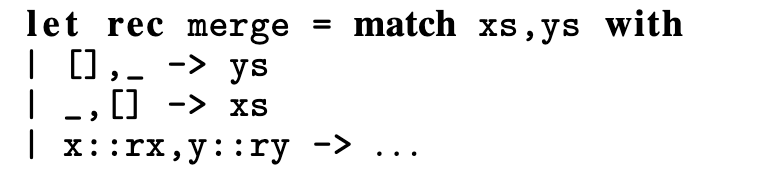
\includegraphics[scale=0.7]{../images/merge.png}
        \Description{Maranget's merge implementation}
        \caption{The skeleton of Maranget's \tt{merge}}
    \end{figure}

    % He then shows an intermediate representation in his compilation algorithm,
    % the occurrence vector and clause matrix: 

    % \begin{figure}[H]
    %     \begin{gather*}
    %         \vec{o} = (\tt{xs ys}) \hspace{3em}
    %         P \rightarrow A = 
    %         \begin{pmatrix}
    %             \tt{[]}     & \tt{\_}     & \rightarrow \tt{xs} \\
    %             \tt{\_}     & \tt{[]}     & \rightarrow \tt{ys} \\
    %             \tt{\_::\_} & \tt{\_::\_} & \rightarrow \tt{...} 
    %         \end{pmatrix}
    %     \end{gather*}


    %     \Description{Occurrence vector of names, and clause matrix of matches}
    %     \caption{The occurrence vector and clause matrix are intermediate
    %     representations in Maranget's compilation. I do not exploit this
    %     representation in my own algorithm, but it helps to understand his final
    %     tree.}
    % \end{figure}

    He compiles the function to this decision tree: 

    \begin{figure}[H]
        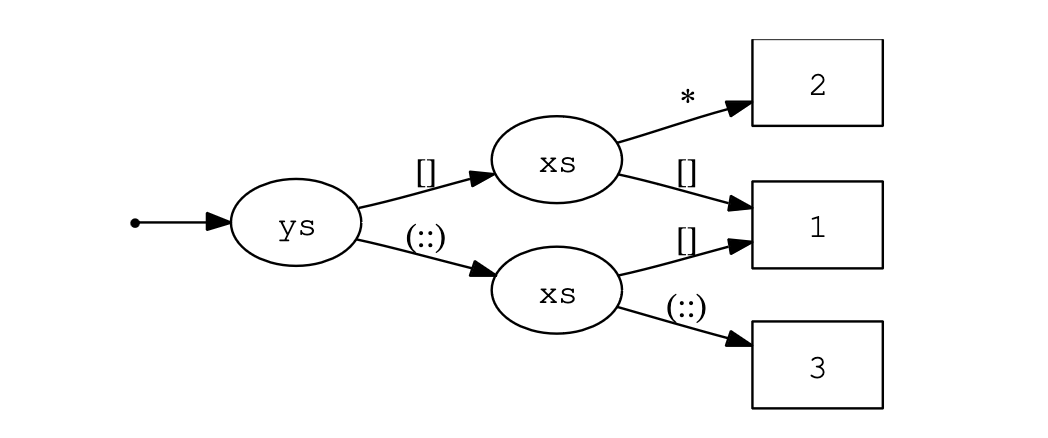
\includegraphics[scale=0.7]{../images/dtree.png}
        \Description{The final decision tree for merge} 
        \caption{The final compiled decision tree for \tt{merge}, right-to-left}
    \end{figure}

    When presented with the values \tt{xs} and \tt{ys}, the tree first tests
    \tt{xs} against its two known possible forms: the nullary list constructor
    \tt{[]}, and the application of the \it{cons} constructor \tt{::}. If
    \tt{xs} is equal to \tt{[]}, the tree immediately returns \tt{ys}. If
    \tt{xs} is an application of \tt{::}, the tree then tests \tt{ys} against
    the same list of possible constructors, and returns a value according to the
    result of the match. Each time the tree goes down a \tt{::} branch, it can
    extract the arguments of the \tt{::} for later use: these are \tt{x},
    \tt{y}, \tt{xr}, and \tt{yr}, which are used in the \tt{...} branch. This
    process of extracting arguments generalizes to all value constructors with
    one or more arguments. 

    \begin{figure}
      \begin{center}
      \dcsyntax
      \end{center}
      \Description{The concrete syntax of D.}
      \caption{\D: Concrete syntax}
      \label{fig:dsyntax}
      \end{figure}

    % Here is the decision tree for \tt{merge} in \D. 

    % \begin{figure}[H]
    %   \centering
    %     \it{Like the semantics, this figure is in progress.}
    %     \Description{The decision tree for merge, now in D} 
    %     \caption{The tree for \tt{merge} in D looks similar to Maranget's.}
    % \end{figure}

    In \D, an \it{extract} node extract all from a value constructor at once for
    use in subtrees. The compiler is responsible for introducing the fresh names
    used in \it{extract}. \VMinus syntax is not closed under substitution during 
    match compilation; this is acceptable because the compiler alpha-renames all
    necessary terms before it translates an \it{if-fi} to a decision tree. 

    In \D, like in \VMinus, expressions can \it{fail}, meaning some of \D's
    syntactic forms like \it{try-let} and \it{cmp} have an extra branch which is
    executed if the examined expression fails. 


    \subsection{Rules (Big-step Operational Semantics) for \D:}
    \label{dsemantics}
    
    \rab{The semantics for \D are being revised.}
    % \dsemantics
    \subsection{The \DTran\ algorithm: \VMinus $\rightarrow$ \D}

    \algrenewcommand\algorithmicwhile{\bf{let }}
    \algrenewcommand\algorithmicdo{\bf{in }}
    \algrenewcommand\algorithmicend{\bf{end}}
    \newcommand\alet\algorithmicwhile
    \newcommand\ain\algorithmicdo
    \newcommand\aend\algorithmicend

    \newcommand\branches{\ensuremath{\mathit{branches}}}
    \newcommand\mg{\ensuremath{-}}


    When presented with an \it{if-fi}, \DTran\ calls the function \Compile,
    whole algorithm is presented in Figure~\ref{dtran}. \DTran\ first introduces
    all the names under the all existential $\exists$'s to a context which
    determines if a name is \it{known} or \it{unknown}. At the start, each name
    introduced by $\exists$ is \it{unknown}. Since all names are unique at this
    stage, there are no clashes. \DTran\ also desugars choice to multiple
    \it{if-fi} branches with a desugaring function \ITran: 

    \itran{if\; \dots \square\; gs_{1};\; \choiceg{gs_{2}}{gs_{3}};\; gs_{4} \rightarrow e\; \square \dots \;fi}
    
    ==
    
    ${if\; \dots \square\; gs_{1};\; gs_{2} \rightarrow e \;\square\; gs_{3};\; gs_{4} \rightarrow e \;\square \dots \;fi}$


    With the new context and desugared \it{if-fi}, \Compile\ then repeatedly
    chooses a guarded expression $G$ and attempts the following while
    translating $G$'s internal expressions with \DTran: 

    \begin{enumerate}
        \item If there are no guards in $G$, insert a \it{match} node with the
        right-hand side of $G$. 
        \item Otherwise, choose an equation in $G$ of the form $x = K \dots$
        s.t. $x$ is \it{known}. 
        \item If one is found, use it to generate a \it{test} node, building
        each subtree of the \it{test} by pruning all branches in \it{all}
        guarded expressions of the \it{if-fi} in which $x = e$ and $e \neq K
        \dots$ and invoking \Compile\ on the remaining ones with a context where
        $x$ is known. Each of these remainders is the child of an \it{extract}
        node which extracts the internals of each possible value constructor
        into a list of names which are introduced to the context. The algorithm
        builds the default tree of the \it{test} by finding any branches of the
        in the \it{if-fi} in which $x$ is not bound to a value constructor. 
        \item If no equation of the form \it{x = K \dots} is found, try to find
        an equation $x = e$ s.t. either $x$ is unknown and all names in $e$ are
        known. 
        \item If one is found, use it to generate a \it{try-let} node with two
        children: one if binding succeeds, and one if $e$ fails. \Compile prunes
        each subtree of the \it{try-let} accordingly.
        \item If no equation is found, try to find an equation $x = y$ s.t. $x$
        is known and $y$ is unknown. 
        \item If one is found, use it to generate a \it{try-let} node with one
        child for when binding succeeds. \Compile prunes the subtree of all 
        instance of $x = y$. 
        \item If no such equation is found, try to find a condition $e$ s.t. all
        names in $e$ are known. 
        \item If one is found, generate a fresh name $x'$ and use it to generate
        a \it{try-let} node for the equation $x = e'$, pruning each subtree of
        $e$ with a substitution of $[x/e]$. 
        \item If no condition $e$ is found, try to find an equation $x = e$ s.t.
        both $x$ and all names in $e$ are \it{known}.
        \item If one is found, generate a \it{cmp} node, prune the \it{if-fi} of
        all duplicate instances of that $x = e$, and invoke \Compile again. 
        \item If none is found, the \it{if-fi} cannot be compiled to a decision
        tree. The algorithm halts with an error. 
    \end{enumerate}
    \raggedbottom

    The algorithm terminates when inserts a final \it{match} node for a
    right-hand side expression $e$ when the list of guards preceding $e$ is
    empty or a list of assignments from names to unbound names. Termination of
    \DTran\ is guaranteed because each recursive call passes a list of guarded
    expressions in which the number of guards is strictly smaller, so eventually
    the algorithm reaches a state in which the first unmatched branch is all
    trivially-satisfied guards. 

    In the figure, I use the notation $x@b$ to denote the bag of all guards and
    expressions in branch $b$ in which name $x$ appears. A branch is a list of
    guards followed by a terminal expression; it is a branch of an \it{if-fi}
    stripped of the existential since \DTran\ introduces all names at the top
    level. I use the notation $\dom(b)$ to describe the set of all names that
    appear in a branch. I use the notation $\mathit{branches -- g}$ to mean
    “$\mathit{branches}$ pruned of guard $g$” and the notation $\mathit{branches
    --- g}$ to mean “$\mathit{branches}$ pruned of all \it{branches} containing
    $g$.” I use the standard substitution notation $\mathit{branches[x/e]}$ to
    mean “$\mathit{branches}$ with name $x$ substituted for expression $e$.” I
    use a shorthand $\mathit{(context + \bracketed{n_1 \dots n_i \mapsto
    known})}$ to mean “$\mathit{context}$ extended with each of $n_x$ bound to
    $\mathit{known}$. 

    Not show in the algorithm is the case where \Compile\ cannot choose a $g$ of
    one of the valid forms; in this case, \Compile\ halts with an error. This
    can happen when no $g$ is currently solvable in the context, as determined
    by the same algorithm that \VMinus uses to pick a guard to solve, or when
    the program would be forced to unify incompatible values, such as any value
    with a lambda. 

    % \DTran\ makes the distinction for an equation \it{x = e}
    % based off of this model: 
    % \begin{enumerate}
    % \item 
    % \end{enumerate}
    % No guards  ==  MATCH
    % CONDITION  ==   if known, convert to LET, IF
    % EQN (x, e) ==
    %    - if x is known and e is VCONAPP, generate TEST
    %    - if x is known and e is not VCONAPP and e is known
    %         generate LET, IF
    %    - if x is unknown and e is known, then generate LET
       
%  What if we don't find any of the above? 
%  There must be only unknown guards. 
%  Can't compile! 
    
    % For an equation that
    % represents a binding of values to values, the algorithm inserts a \it{let}
    % node, and for a condition guard \it{e}, it inserts a \it{let} followed by 
    % an \it{if-then-else}. 
    
  
    \begin{figure}[H]
      \scriptsize

      sdf

%       \begin{algorithmic}
% \Require $\forall (n : \rm{name})\; \in \branches, \; n\; \rm{unique}$
% \State \it{compile context \branches} = 
%   \If{\it{null(\branches)}} {\it{fail}}
%   \ElsIf{$\neg\exists{g} \in$ \it{fst(hd(\branches))}} 
%     \State {\it{match (hd branches)}}
%   \Else
%     \State \alet $g$ be a guard such that $g \in \branches$
%     \ain 
%     \If{$g$ has the form $x = K (e_1 \dots e_i)$}
%     \alet 
%     \State 
%     $\mathit{KS = \bracketed{K\; \vert\; \exists\; b \in \branches : x \in \dom(b) \wedge K(\dots) \in x@b }}$ 
        
%     $\mathit{edges = map(}$ 
%     \State $\mathit{\lambda K.}$ (\alet $ns = n_1 \dots n_i, \; n_x \rm{ fresh}$
%         \ain 
%         \State $\mathit{(K, extract (x, ns, \Compile (context + \bracketed{n_1 \dots n_i \mapsto known})}$ 
%         \State $\mathit{(mapPartial (refine\; x\; (K (ns))) branches))}$ 
%         \State \aend) 
%       \State $\mathit{defaults = filter(\lambda b. x \notin \dom(b) \lor K(\dots) \notin x@b)}$ 
%       \State \ain $\mathit{test (x, edges, SOME (compile\; defaults))}$ 
%       \State \aend 
%     \ElsIf {$g$ has the form $x = e$ : $x \;\mathit{unknown},\; e \;\mathit{known}$} 
%       \State $\mathit{try\_let (x, \DTran\; (context\; e)}$, 
%       \State $\mathit{compile (context\bracketed{x \mapsto known}) ((branches -- eq)[x/e])}$,
%       \State $\mathit{SOME (compile\; context\; (branches --- eq --- e)))}$
%     \ElsIf {$g$ has the form $x = y$ : $x \;\mathit{known},\; y \;\mathit{unknown}$} 
%     \State $\mathit{try\_let (x, y, compile (context\bracketed{y \mapsto known}) (branches -- eq), NONE)}$
%     \ElsIf {$g$ has the form $x = e$ : $x \;\mathit{known},\; e \;\mathit{known}$} 
%       \State $\mathit{cmp (x, \DTran\; (context\; e)}$, 
%       \State $\mathit{compile\; context\; ((branches -- eq)[x/e])}$,
%       \State $\mathit{compile\; context\; (branches --- eq -- e)}$,
%       \State $\mathit{SOME (compile\; context\; (branches --- eq --- e)))}$
%     \ElsIf {$g$ has the form $e$ : $e \;\mathit{known}$} 
%     \State $\mathit{try\_let (x, \DTran\; (context\; e)}$, 
%     \State $\mathit{compile (context\bracketed{x \mapsto known}) ((branches -- eq)[x/e])}$,
%     \State $\mathit{SOME (compile\; context\; (branches --- eq --- e)))}$ 
%     \State {, $x$ fresh} \\
%     \aend
%     \EndIf
%   \EndIf
%   \State \bf{where} 
%   \State $\mathit{snd (a, b) = b}$ 
%   \State $\mathit{refine (x, K (ns) b) = }$
%   \If{$\mathit{K' (es) \in x@b \land (K \neq K' \lor length(es) \neq length(ns))}$}
%         $\mathit{NONE}$
%   \Else $\;\mathit{SOME\; b}$
%   \EndIf 

% \end{algorithmic}


\Description{The \DTran\ algorithm} 
    \caption{The \DTran\ algorithm.}
    \label{dtran}
    \end{figure}    



    \subsection{Translation from \VMinus to \D preserves semantics}
    
    Translating \it{if-fi} to a decision tree should preserve semantics. The
    following theorem formalizes this claim: 

    \begin{proof}
        See appendix A. 
    \end{proof}

\end{document}
\documentclass[manuscript,screen,review, 12pt, nonacm]{acmart}
\let\Bbbk\relax % Fix for amssymb clash 
\usepackage{vmlmacros}
\AtBeginDocument{%
  \providecommand\BibTeX{{%
    \normalfont B\kern-0.5em{\scshape i\kern-0.25em b}\kern-0.8em\TeX}}}
\usepackage{outlines}
\setlength{\headheight}{14.0pt}
\setlength{\footskip}{13.3pt}
\title{An Alternative to Pattern Matching, Inspired by Verse}

\author{Roger Burtonpatel}
\email{roger.burtonpatel@tufts.edu}
\affiliation{%
\institution{Tufts University}
\streetaddress{419 Boston Ave}
  \city{Medford}
  \state{Massachusetts}
  \country{USA}
  \postcode{02155}
  }
\begin{document}
\section{Equations subsume pattern matching with popular extensions}
\label{pplustovminus}
    In my introduction I stated that \VMinus can be compiled to a decision
    tree, and that \VMinus subsumes pattern matching with popular extensions.
    Having proved the former, I now prove the latter. I do so by showing an
    algorithm \PtoVTran\ which translates \PPlus to \VMinus, and proving that
    the translation preserves semantics. 

    \subsection{Domains}

    I give the names and domains of the translation functions: 
    
    \begin{align*}
        &\PtoVTran: \PPlus Exp\; \rightarrow\; \VMinus Exp \\
        &\PTran: Pattern\; \rightarrow\; Name\; \rightarrow\; Name\ list\ *\ Guard\ list \\
        % &\mathcal{B}: Pattern\; ->\; Name\; Set \\
    \end{align*}
    
    The translation functions \PtoVTran\ and \PTran\ are defined case by case: 
    
    % \subsection{Binding names}
    
    % \begin{align*}
        %     &\Bindings{x} = \bracketed{x} \\ 
        %     &\Bindings{K} = \bracketed{} \\
        %     &\Bindings{K\; p_{1} {\dots} p_{n}} = \Bindings{p} \cup {\dots} \cup \Bindings{p_{n}} \\
        %     &\Bindings{\porp} = \Bindings{p_{1}} \cap \Bindings{p_{2}} \\
        %     &\Bindings{\pcommap} = \Bindings{p} \cup \Bindings{p'} \\
        %     &\Bindings{\parrowe} = \Bindings{p} \\
        %     &\Bindings{\whenexpr} = \bracketed{}
        % \end{align*}
        
        \subsection{Translating Expressions}
        
        \newcommand\btran[1]{\mathcal{B}[\![#1]\!]}
        
        \begin{align*}
            &\ptov[exp=x, result=x] \\
            &\ptov[exp={K\; \expr[1] {\dots} \expr[n]}, result={K\; \ptovtran{\expr[1]} {\dots} \ptovtran{\expr[n]}}] \\
            &\ptov[exp={\lambda x.\; \expr}, result={\lambda x.\; \ptovtran{\expr}}] \\
            &\ptov[exp={\expr[1]\; \expr[2]}, result={\ptovtran{\expr[1]}\; \ptovtran{\expr[2]}}] \\
            % &\ptov[exp={\tt{case}\; \expr\;  \emptyseq}, result={{\iffitt{\vexists{x}\; x = \ptovtran{\expr};\; \iffitt{}}}}]\; \rm{, $x$ fresh }   \\
            &\ptovtran{\tt{case}\; \expr\;  p_{1}\; \expr[1] \vert {\dots} \vert p_{n}\; \expr[n]} \rightsquigarrow \\
            &\hspace{2em} \rm{$\forall i.\; 1 \leq i \leq n:$} \\
            &\hspace{2em} \tt{if } {\vexists{x}\; x \tt{ = } \ptovtran{\expr};}\; \\
            &\hspace{2em} \rm{ let } (\mathit{ns}_{1}, \mathit{gs}_{1}) {\dots} (\mathit{ns}_{i}, \mathit{gs}_{i}) = \ptran{p_{1}}x\; \cdot\; {\dots} \cdot\; \ptran{p_{i}}x \rm { in } \\
            &\hspace{2em} \iffitt{\vexists{\mathit{ns}_{1}}\; {\mathit{gs}_{1}} \rightarrow \ptovtran{\expr[1]};\;
                       \square\; {\dots} \square\; \vexists {\mathit{ns}_{i}}\; {\mathit{gs}_{i}} \rightarrow \ptovtran{\expr[i]}} \\
            &\hspace{2em} \tt{fi} \\
            &\hspace{2em} \rm{, $x$ fresh }
        \end{align*}
        
        \subsection{Translating Patterns}
        
        \begin{align*}
            &\pattov[pat=y, result={(y, [x = y])}] \\
            &\pattov[pat=K, result={([], [x = K])}] \\
            &\ptran{K\; p_{1}\; {\dots}\; p_{n}}x \rightsquigarrow \\
            &\hspace{2em} \rm{$\forall i.\; 1 \leq i \leq n:$} \\
            &\hspace{2em} \rm{ let } y_{i} \rm{ be a fresh name, }  \\
            &\hspace{2em} (\mathit{ns}_{1}, \mathit{gs}_{1}) {\dots} (\mathit{ns}_{i}, \mathit{gs}_{i}) = \ptran{p_{1}}y_{1} \cdot {\dots} \cdot \ptran{p_{i}}y_{i} \\
            &\hspace{2em} \rm{ in } \\
            &\hspace{2em} ({\mathit{ns}_{1} \cdot {\dots} \cdot \mathit{ns}_{i}} \cdot {y_{1} {\dots} y_{i}}, x = K\; y_{1}\; {\dots}\; y_{i} \cdot \; \mathit{gs}_{1} \cdot {\dots} \cdot \mathit{gs}_{i}) \\
            &\pattov[pat=\mathit{when}\; e, result={([], [\ptovtran{e}])}] \\
            &\pattov[pat=\pcommap, 
            result={\rm{let } 
            {(\mathit{ns}_{1}, \mathit{gs}_{1}) = \ptran{p}x}\; , 
            {(\mathit{ns}_{2}, \mathit{gs}_{2}) = \ptran{p'}x} \rm{ in }
            (\mathit{ns}_{1} \cdot \mathit{ns}_{2}, \mathit{gs}_{1} \cdot \mathit{gs}_{2})}] \\
            &\pattov[pat=\porp, 
            result={\rm{let } (\mathit{ns}_{1}, \mathit{gs}_{1}) = \ptran{p}x\; ,
            (\mathit{ns}_{2}, \mathit{gs}_{2}) = \ptran{p'}x \rm{ in }
            (\mathit{ns}_{1} \cdot \mathit{ns}_{2}, [\mathit{gs}_{1} \choice \mathit{gs}_{2}])}]
        \end{align*}
        

        \rab{Questions: What notes do you have on the formatting? How is my use
        of oxford brackets? Do you see any obvious places to insert or remove
        them?}

    To compile \it{case} expressions to decision trees like Maranget does,
    translate \PPlus to \D using $(\DTran\; o\; \PtoVTran)$.
    
    Finally, I claim that the translation from \it{case} expressions to decision
    trees, $(\DTran\; o\; \PtoVTran)$, is consistent with Maranget and
    others~\citep{maranget,scottramsey}. Proving this claim is a good goal for
    future work; it is not the main focus of this paper. 

    \section{Related Work}

    The dual foundations of this paper are Augustsson et al.'s Verse
    Calculus~\citep{verse} and Maranget's decision trees~\citep{maranget}.
    Augustsson et al. give the formal rewrite semantics for the Verse Calculus;
    Maranget gives an elegant formalism of decision trees. 
    
    Extensions to pattern matching, and how they appeal to language designers,
    find an excellent example in Erwig \& Peyton Jones~\citep{guardproposal}.
    
    Compiling Pattern Matching~\citep{augustsson1985compiling} by Augustsson
    gives a foundation in exactly what it says. Ramsey and Scott have a crisp
    example of a match-compilation algorithm (pattern matching to decision
    trees) in When Do Match-Compilation Heuristics Matter?~\citep{scottramsey}. 
    
    \section{Future Work}        
    \label{futurework}
        \subsubsection{Typing \PPlus and \VMinus}
        \label{typingppandvm}

        I have described how a type system for both \PPlus and \VMinus is a
        worthwhile effort. Notably, a type system can help restore Nice Property
        5: with a type system, the compiler can warn programmers of a missing or
        extraneous match condition in a \it{case} expression, and potentially an
        \it{if-fi}. Owing to its significantly more flexible structure, however,
        \it{if-fi} may prove trickier to analyze for missing match conditions
        than \it{case}.

        \subsubsection{Type-agnostic decision-making: the $\alpha$}
        \label{alphas}

        The three languages look similar: they each have value constructors and
        a 'decision-making construct' to deal with constructed data. In \PPlus, the
        construct is pattern-matching; in \VMinus, it is the guarded expression; in \D,
        it is the decision tree. 

        Because of this, it might be possible to make all three languages
        \it{higher order} in right-hand sides; that is, to parameterize the
        expressions that occur \it{after} all decision-making. Imagine an
        abstract expression $\alpha$ that appears on the right-hand side of a
        \it{case} branch, the right-hand side of a guarded expression, or in a
        \it{match} node. The abstract syntax of the new \it{case}, \it{if-fi},
        and decision tree might look like this: 
        \begin{center}
            \begin{bnf}
                $\VMinus_{\alpha}$ : \VMinus with $\alpha$ ::=
                $\mathit{if}\; \mathit{[}\; g\; \bracketed{[] g}\; \mathit{]}\; \mathit{fi}$ : if-fi with $\alpha$
                ;;
                $G_{\alpha}$ : Guarded Expressions with $\alpha$ ::=
                $[\vexists{\bracketed{x}}] \bracketed{g} \boldsymbol{\rightarrow}\alpha$ : 
                ;;
                $\PPlus_{\alpha}$ : \PPlus with $\alpha$::=
                $\tt{case}\; \expr\; \bracketed{p\; \ttrightarrow\; \alpha}$ : \it{case} expression with $\alpha$ 
                ;;
                $t_{\alpha}$ : Decision Trees with $\alpha$ ::= 
                | \dots : other forms of tree 
                | $\alpha$ : match node 
            \end{bnf}
        \end{center}

        Why would one want to do this? Well, recall that \VMinus had to be
        stripped of multiple results and other \VC-like constructs in order to
        retain its desirable efficiency properties. $\alpha$ lets \VMinus and
        the other languages do efficient decision-making without worrying about
        the form of the result. If the result is a complex multi-value or a
        computation that involves backtracking, it will be agnostic of the
        decision-making. $\alpha$ makes right-hand sides polymorphic and
        abstract, so a programmer could potentially insert expressions from \VC
        in their place and know that the decision-making before the $\alpha$
        will still be efficient. This would allow for fuller interoperability
        between \VC and \VMinus. Section~\ref{vminusandvc} further describes
        why bridging the gap between the two languages might be a worthwhile
        exercise. 

        However, the language designer must take special care to ensure no
        $\alpha$ finds its way into the decision-making itself, or the whole
        idea falls apart. I am developing an implementation that enforces this
        invariant, and may include it in a future publication. 
        
        % Other alpha material: 
% The decision-making construct that gets us there. Whether
% it's a single value (ML-style) a sequence of values (Verse-style), or
% even something else, the $\alpha$ represents \it{any} ultimate result of
% "making a decision," and it's the ways in which we make decisions that
% we truly care about examining. By making the return result both
% polymorphic and abstract, we eschew the need to worry about its type and
% compatibility with other results of otherwise-equivalent trees. 

% An expression in core Verse evaluates to produce possibly-empty sequence of
% values. In \VMinus, values depend on the form of abstract expression $\alpha.$
% If $\alpha$ is a Verse-like expression, \valpha\ will be a value sequence. If it
% is an ML-like expression, it will be a single value. 
            
%         A guarded expression evaluates to produce a \bf{result}. A result is either
%         a metavalue \valpha\ or reject. 
            
%         \[\it{r}\; \rm{::=}\; \vartheta\; \vbar \; \reject \]
            
%         \showvjudgement{Eval-Alpha}{\veval{\alpha}{\valpha}}

% Of note in both \VMinus and \D is that the 'decision-making construct'
% is annotated with an $\alpha$. This annotation gives us type flexibility on the
% right-hand side of the \it{terminating} case for each construct
% (\tt{$\rightarrow$ exp} in \VMinus and the match node in \D.) 


        \subsubsection{Studying \PPlus independently}
        \label{pplusindependently}
        \PPlus has side conditions, guards, and or-patterns. No major
        functional language has all three of these extensions. Back
        Section~\ref{extensions}'s examples, I had to switch from OCaml to
        Haskell to use guards, and back to OCaml for or-patterns. The two
        extensions are mutually exclusive in Haskell, OCaml, Scala,
        Erlang/Elixir, Rust, F\#, Agda.~\citep{haskell, ocaml, scala, erlang,
        elixir, rust, fsharp, agda}

        I have yet to encounter a substantial justification for this. I have
        several theories: one, reengineering the Haskell parser to integrate
        or-patterns into the language may be considered too great an effort;
        two, the lesser popularity of functional programming in comparison to
        other paradigms has meant there are not enough voices in any one
        language's community claiming that theirs needs all known extensions to
        pattern matching; three, the most efficient algorithms for compiling the
        three extensions are somehow incompatible. Future work may explore if
        efficient compilation of \PPlus is possible; such a study may answer this
        question. 

        \subsubsection{Using \VMinus to inform programming in Verse}
        \label{vminusandvc}
        
        At ICFP last year, Tim Sweeney said that he wanted Verse to be an
        accessible programming language to write a scalable, collaborative
        metaverse~\citep{timtalk}. Can \VMinus be aid in this goal? I can imagine
        two ways in which it might:
        
        \begin{enumerate}
            \item \VMinus could be  a tool to help ease programmers who are
            more familiar with pattern matching into the realm of functional
            logic programming with equations. 
            \item Programs written in Verse using ideas from \VMinus might have
            a friendlier cost model (depending on the compiler)
        \end{enumerate}
        
        To point~1, \VMinus sits both syntactically and semantically in between
        \PPlus and \VC, which might help a new programmer to Verse bridge the
        conceptual gap between pattern matching and equations. Also, \PtoVTran,
        the $\PPlus \rightarrow \VMinus$ translation, could help a programmer 
        who wishes to write code using pattern matching see how their ideas 
        can be expressed in Verse. 

        To point~2, \DTran\ and the proof that \DTran\ preserves semantics help
        show that certain computations that use equations for decision-making
        can be compiled to efficient code. My hope is that, using these ideas,
        both the Verse programmer and language designer might make any discovery
        that allows them to increase the efficiency of full-Verse programs. 

    \section{Conclusion}

    I have introduced the languages \PPlus and \VMinus to explore the design
    space of pattern matching and equations, and \D, \PtoVTran, and \DTran\ to
    show how these languages can make decisions efficiently. 

    The languages are made for use and experimentation: they are syntactically
    simple and have conceptually accessible operational semantics. I hope that
    programmers will explore and develop their own opinions of these languages,
    which are publically available at
    \url{https://github.com/rogerburtonpatel/vml}. 

    Finally, and in particular with \VMinus, I hope to have paved a small
    segment of the path that the curious programmer or language enthusiast who
    wishes to better understand Verse will take. Be they transitioning to
    equations from pattern matching to equations or curious about how those
    equations might be compilable to decision trees, I hope they find the
    languages, and this document, illuminating. 
    
\end{document}
\documentclass[manuscript,screen,review, 12pt, nonacm]{acmart}
\let\Bbbk\relax % Fix for amssymb clash 
\usepackage{vmlmacros}
\AtBeginDocument{%
  \providecommand\BibTeX{{%
    \normalfont B\kern-0.5em{\scshape i\kern-0.25em b}\kern-0.8em\TeX}}}
\usepackage{outlines}
\setlength{\headheight}{14.0pt}
\setlength{\footskip}{13.3pt}
\title{An Alternative to Pattern Matching, Inspired by Verse}

\author{Roger Burtonpatel}
\email{roger.burtonpatel@tufts.edu}
\affiliation{%
\institution{Tufts University}
\streetaddress{419 Boston Ave}
  \city{Medford}
  \state{Massachusetts}
  \country{USA}
  \postcode{02155}
  }
\begin{document}

\section{Acknowledgements}

This thesis would not have been possible without the infinitely generous time
and support of my advisors, Norman Ramsey and Milod Kazerounian. Norman's
offhand comment of “I wonder if Verse's equations subsume pattern matching” was
the entire basis of this work, and his generosity in agreeing to advise a full
thesis to answer his question will always be profoundly appreciated. During the
academic year, Norman provided me with materials on both the technical story and
on how to write about it well. He gave me regular feedback and has helped
improve my research skills, my technical writing, and my understanding of
programming languages in general tremendously. I especially appreciate how he
has guided me in-person at the end of my undergraduate when his book~\citep{bpc}
got me started down the path of PL at the beginning of it. Finally, Norman is
also fantastically fun to pair program with. 

From the beginning, Milod provided me with encouraging mentorship that kept
me enthusiastic and determined to complete the project. He was exceptionally
patient as I gave him whirlwind tour after whirlwind tour of the changing
codebase and problems, and kept me grounded in the problems at hand. He 
sent me helpful examples of his research to aid me in my proofs, and gave me
some particularly encouraging words towards the end of the project that I 
will not soon forget. 

My undergraduate advisor, Mark Sheldon, has always been both supportive and
kind. I have enjoyed many long talks in his office, and I am deeply grateful
that he is on my committee. 

Alva Couch was the advisor of my original thesis idea, which was to compile
programming languages with music. Ultimately, we decided that I should pursue
this project instead, and I am grateful to him for his mentorship in that moment
and onwards. 

My family--- my mother, Jennifer Burton, my father, Aniruddh Patel, and my
sister, Lilia Burtonpatel, have all given me support, encouragement, and
(arguably most importantly) food. My gratitude for them is immeasurable. 

My gratitude towards my friends is also without limit. In particular, and in
no order, Liam Strand, Annika Tanner, Max Stein, Cecelia Crumlish, and
Charlie Bohnsack all showed specific interest in the work and encouraged me
as I moved forward. Rachael Clawson was subjected to much rubber-ducking,
and endured valiantly. Aliénor Rice and Marie Kazibwe were as steadfast
thesis buddies as I could ever hope for. Jasper Geer, my PL partner in
crime, was always one of my favorite people to talk to about my thesis. His
pursuits in research inspire mine. 

Skylar Gilfeather, my unbelievable friend. Yours is support that goes
beyond words; care, food, silent and spoken friendship, late night rides to
anywhere, laughs and tears are some that can try to capture it. I am so, so
grateful for how ceaselessly you've encouraged me on this journey. Every one
of your friends is lucky to have you in their life, and I am blessed that 
you are such a core part of mine. 

Anna Quirós, I am writing these words as you sleep behind me. Your support
and love have been immeasurable. I will always be grateful to you for this
year \it{increíble}. I could not have smiled through it all without you. 

Thank you all. 

\section{References}
\bibliographystyle{ACM-Reference-Format}
\bibliography{sources}

\renewcommand\thesection{\Alph{section}}
\setcounter{section}{0}
\section{Proofs}
\begin{outline}
\1 \bf{Proof: Translation from \VMinus to \D\ preserves semantics }
\1 \bf{Proof: Translation from \PPlus\ to \VMinus preserves semantics }
% \1 \bf{Proof: Translation from \VMinus to Verse preserves semantics}
\end{outline}

\section{Addressing how \PPlus handles unusual pattern combinations}
\label{ppweird}
    \PPlus admits of strange-looking patterns: consider \tt{Cons (when true)
    zs}. But these should not be alarming, because such syntactic forms reduce
    to normal forms by (direct) application of algebraic laws: 

    \begin{align}
      K (\whenexpr) \;p2\; \dots &=== K \;\_ \;p2\; \dots, \whenexpr \\
      K (\whenexpr, \;p2\;) \;p3\; \dots  &=== K \;p2\; \;p3\; \dots, \whenexpr \\
      K (p1\;, \whenexpr) \;p3\; \dots  &=== K \;p1\; \;p3\; \dots, \whenexpr \\
      K (\whenexpr \pbar p2\;) \;p3\; \dots &=== (K \;\_ \;p3\; \dots, \whenexpr) \pbar (K \;p2\; \;p3\; \dots) \\
      K (p1 \pbar \whenexpr) \;p3\; \dots &=== (K \;p2\; \;p3\; \dots) \pbar (K \;\_ \;p3\; \dots, \whenexpr)  \\
      \whenexpr \leftarrow e &=== \;\_ <- e, \whenexpr
    \end{align}   
    
    Repeatedly applying these laws until the program reaches a fixed point
    normalizes placements of \it{when}. Laws (2) and (3) work because \PPlus
    has no side effects and the laws assume all names are unique (the compiler
    takes care of this), so changing the order in which patterns match has no
    effect on semantics.         

\section{Is \VMinus\ a true subset of \VC?}
\VMinus\ certainly appears to relate to \VC\ semantically. Translating
\it{if-fi} and choice in \VMinus to \bf{one} and choice in \VC\ is likely a
sufficient embedding. Formalizing this translation and, more importantly,
proving that our semantics of \VMinus are consistent with Augutsson et al.'s
\VC\ is an excellent goal for future work. 

\section{Formal Definitions of all languages}
\label{languagedefs}

\utable
\ppsemantics
\vmsemantics

% \begin{figure}
% \begin{center}
%     \begin{bnf}
%     $P$ : \textsf{Programs} ::=
%     $\bracketed{d}$ : definition
%     ;;
%     $d$ : \textsf{Definitions} ::=
%     | $\tt{val}\; x\; \tt{=}\; \expr$ : bind name to expression
%     ;;
%     $\expr$ : \textsf{Expressions} ::=
%     | $v$ : literal values 
%     | $x, y, z$ : names
%     | $\tt{if}\; [\; G\; \bracketed{\tt{[]}\; G}\;]\; \tt{fi}$ : if-fi 
%     | $K \bracketed{\expr}$ : value constructor application 
%     | $\expr[1]\; \expr[2]$ : function application 
%     | $\ttbackslash x\tt{.}\; \expr$ : lambda declaration 
%     ;;
%     $G$ : \textsf{Guarded Expressions} ::=  
%     $[\tt{E }{\bracketed{x}}{\tt{.}}] \bracketed{g} \;\ttrightarrow\; \expr$ : names, guards, and body
%     ;;
%     $g$ : \textsf{Guards} ::=  
%     | $\expr$ : intermediate expression 
%     | $x \;\tt{=}\; \expr$ : equation 
%     | $ g \bracketed{\tt{;} g} \; \pbar \; g \bracketed{\tt{;} g}$ : choice 
%     ;;
%     $\v$ : Values ::= $K\bracketed{\v}$ : value constructor application 
%     | $\ttbackslash x\tt{.}\; \expr$ : lambda value
%     \end{bnf}
% \end{center}
% \Description{The concrete syntax of PPlus.}
%     \caption{\VMinus: Concrete syntax}
%     \label{fig:vmsyntax}
%     \end{figure}

% \begin{figure}
%     \begin{center}
%     \begin{bnf}
%     $P$ : \textsf{Programs} ::=
%     $\bracketed{d}$ : definition
%     ;;
%     $d$ : \textsf{Definitions} ::=
%     | $\tt{val}\; x\; \tt{=}\; \expr$ : bind name to expression
%     ;;
%     $\expr$ : Expressions ::= 
%     | $v$ : literal values 
%     | $x, y, z$ : names
%     | $K\bracketed{\expr}$ : value constructor application 
%     | $\ttbackslash x\tt{.}\; \expr$ : lambda declaration  
%     | $\expr[1]\; \expr[2]$ : function application 
%     | $\tt{case}\; \expr\; \bracketed{p\; \ttrightarrow\; \expr}$ : case expression 
%     | \ttbraced{$\expr$}
%     ;;
%     $p$ : \textsf{Patterns} ::= $p_{1}\pbar p_{2}$ : or-pattern
%     | $p \tt{,} p'$ : pattern guard 
%     | $p\; \tt{<-}\; \expr$ : pattern from explicit expression  
%     | $x$ : name 
%     | $\tt{\_}$ : wildcard 
%     | $K\; \bracketed{p}$ : value constructor application 
%     | $\tt{when}\; \expr$
%     | \ttbraced{$p$}
%     ;;
%     $\v$ : Values ::= $K\bracketed{\v}$ : value constructor application 
%     | $\ttbackslash x\tt{.}\; \expr$ : lambda value 
%     ;;
%     $K$ : \textsf{Value Constructors} ::=
%     | $\tt{true}\; \vert\; \tt{false}$ : booleans
%     | $\tt{A-Z}x$ : name beginning with capital letter
%     % | $[\tt{-}\vert\tt{+}](\tt{0}-\tt{9})+$ : signed integer literal 
%     \end{bnf}
%     \end{center}
%     \Description{The concrete syntax of PPlus.}
%     \caption{\PPlus: Concrete syntax}
%     \end{figure}

\end{document}


\end{document}
\endinput
%%
